\section{Wireframe}\label{s:wireframe}
La realizzazione dei wireframe è stata fatta mediante il software \textit{Balsamiq}; la loro realizzazione ha attraversato diverse iterazioni. Nelle seguenti sezioni presenteremo i vari wireframe e i widget che li compongono spiegando quali sono stati i nostri ragionamenti e le nostre iterazioni per raggiungere la versione finale.\\

\subsubsection{Header e footer}\label{ss:header-e-footer}
Ogni schermata possiede un header nella parte alta dello schermo e un footer nella parte bassa. I footer sono tutti uguali, gli header sono simili in quanto presentano tutti un selettore di data, l'unico che differisce è quello della schermata ``Analisi di periodi'' che ne presenta due in quanto in quella schermata deve essere possibile, per il giornalista, inserire due range di date.

\begin{figure}[H]
    \centering
    
\includegraphics[width=1\columnwidth]{wireframes/header-una-data}
    \caption{Header di ``Panoramica'', ``Confronto fra regioni'' e ``Distribuzione su dati anagrafici''.}\label{fig:header-una-data}
\end{figure}

\begin{figure}[H]
    \centering
    
\includegraphics[width=1\columnwidth]{wireframes/header-due-date}
    \caption{Header di ``Analisi di periodi''.}\label{fig:header-due-date}
\end{figure}

Gli headers sono composti, partendo da destra:
\begin{itemize}
    \item logo della protezione civile;
    \item titolo della dashboard;
    \item pulsante per aprire il menù per selezionare quali widget visualizzare;
    \item pulsante per salvare in locale la vista e l'organizzazione della schermata aperta in quel momento;
    \item pulsante per caricare, e aprire, una schermata, e la sua organizzazione, salvata in precedenza o condivisa da un altro utilizzatore della dashboard;
    \item selettore di date (due in~\ref{fig:header-due-date}) composto da:
        \begin{itemize}
            \item freccia a sinistra, un bottone per passare al giorno precedente a quello indicato;
            \item bottone per aprire il widget per selezionare la data (~\ref{fig:selettore-data-singola} e~\ref{fig:selettore-range-date});
            \item freccia a destra, simile alla freccia a sinistra ma con comportamento opposto, cambia la data al giorno successivo rispetto a quello indicato (se la data è valida).
        \end{itemize}
\end{itemize}

\begin{figure}[H]
    \begin{subfigure}[b]{0.5\textwidth}
        \centering
        
\includegraphics[width=0.4\textwidth]{wireframes/selettore-data-singola}
        \caption{Pulsante per aprire il widget per selezionare una data singola.}\label{fig:selettore-data-singola}
    \end{subfigure}
\hfill
    \begin{subfigure}[b]{0.5\textwidth}
        \centering
        
\includegraphics[width=0.5\textwidth]{wireframes/selettore-range-date}
        \caption{Pulsante per aprire il widget per selezionare un range di date.}\label{fig:selettore-range-date}
    \end{subfigure}
    \caption{Pulsanti per aprire i widget per selezionare una data o un range di date.}
\end{figure}

\begin{bclogo}{Header}
Le prime versione dell'header erano sprovviste del bottone per inserire le metriche e i nomi delle pagine erano differenti.~\ref{fig:header-vecchio} mostra lo stato dell'header prima che aggiungessimo il selettore delle metriche, prima ogni box aveva un pulsante con una ghiera che, al click, apriva la lista di possibile metriche visionabili in quel box. Mentre, i nomi delle schermate sono state cambiate per rendere più semplice capire quali contenuti contengono.
Inoltre il pulsante per aprire il widget per selezionare la data era poco riconoscibile e, in successive iterazioni è stato sistemato anche questo problema.
\begin{figure}[H]
    \centering
    
\includegraphics[width=1\columnwidth]{wireframes/header-vecchio}
    \caption{Prima versione dell'header.}\label{fig:header-vecchio}
\end{figure}
\end{bclogo}

\paragraph{Seleziona metriche}
Il pulsante ``Seleziona metriche'' è stato aggiunto per permettere all'utilizzatore della dashboard di selezionare quali metriche vuole avere all'interna dall schermata. Al suo click compare una lista (\ref{fig:seleziona-metriche}) con tutte le metriche disponibili per quella schermata; l'utente può trascinare una metrica dalla lista all'interno della schermata e rilasciarla in una posizione compatibile andando così a sostituire una delle metriche presenti. Le posizioni compatibili con la metrica trascinata vengono evidenziate in quanto le uniche a colori e con una griglia attorno. Una metrica già presente all'interno della schermata, indicata da una spunta (\checkmark) non sono trascinabili all'interno della schermata, e, in caso di tentativo viene mostrato un avviso all'utente. In caso l'utente clicchi semplicemente su una metrica invece di trascinarla, compare un tooltip sulla metrica cliccata che spiega il funzionamento della meccanica (\ref{fig:seleziona-metriche-tooltip}). \`E in oltre presente un pulsante per ripristinare la schermata alle metriche di default, questo pulsante ha l'etichetta ``Ripristina le metriche di default''.

\begin{figure}[H]
    \begin{subfigure}[b]{0.5\textwidth}
        \centering
        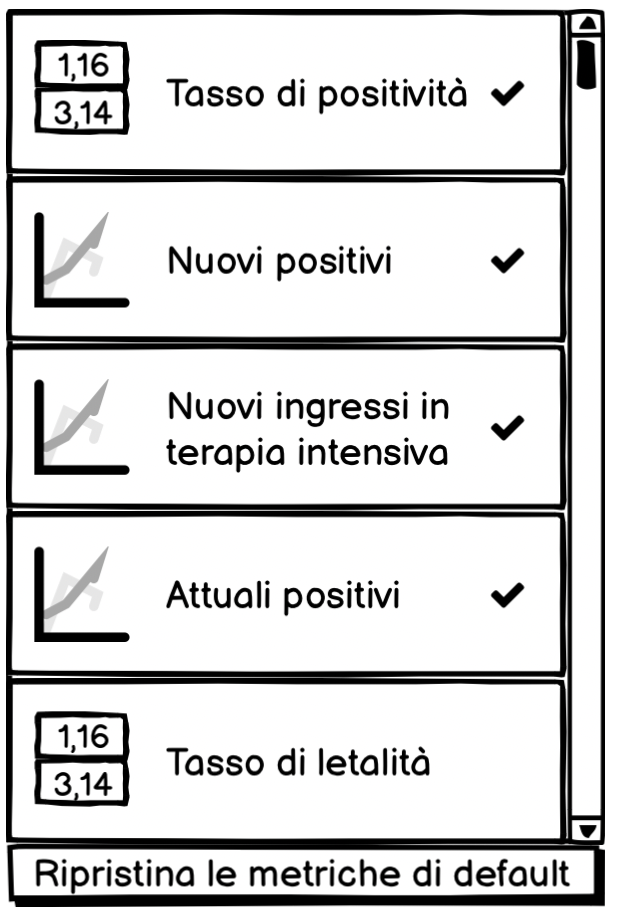
\includegraphics[width=0.3\textwidth]{wireframes/seleziona-metriche}
        \caption{Menù di selezione delle metriche.}\label{fig:seleziona-metriche}
    \end{subfigure}
\hfill
    \begin{subfigure}[b]{0.5\textwidth}
        \centering
        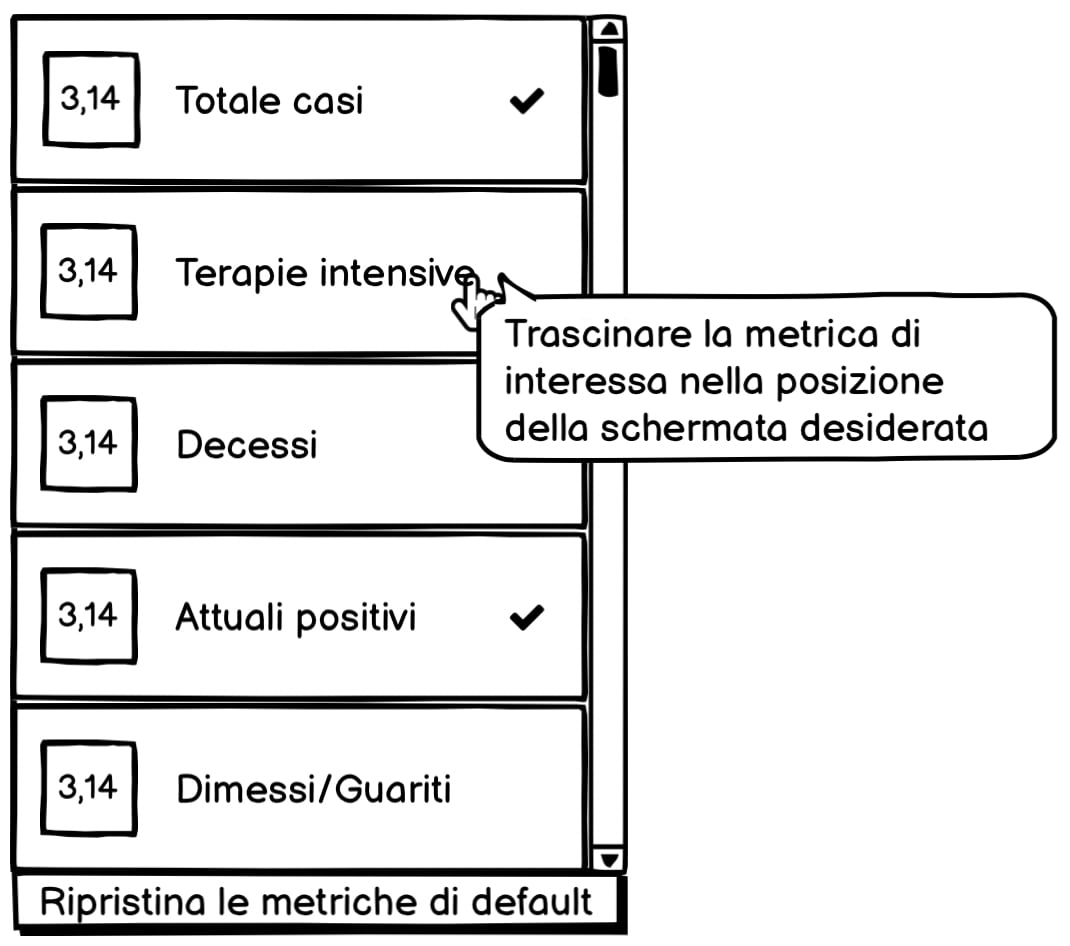
\includegraphics[width=0.5\textwidth]{wireframes/seleziona-metriche-tooltip}
        \caption{Tooltip in caso di click su un elemento della lista.}\label{fig:seleziona-metriche-tooltip}
    \end{subfigure}
    \caption{Seleziona metriche.}
\end{figure}


\paragraph{Seleziona data}
I widget per selezionare la data, apribili tramite il bottone tra le due frecce, sono di due tipi. Uno se la pagina richiede  d'inserire un singolo giorno e l'altro se la pagina richiede d'inserire un range di date.\\

\begin{figure}[H]
    \begin{subfigure}[b]{0.5\textwidth}
        \centering
        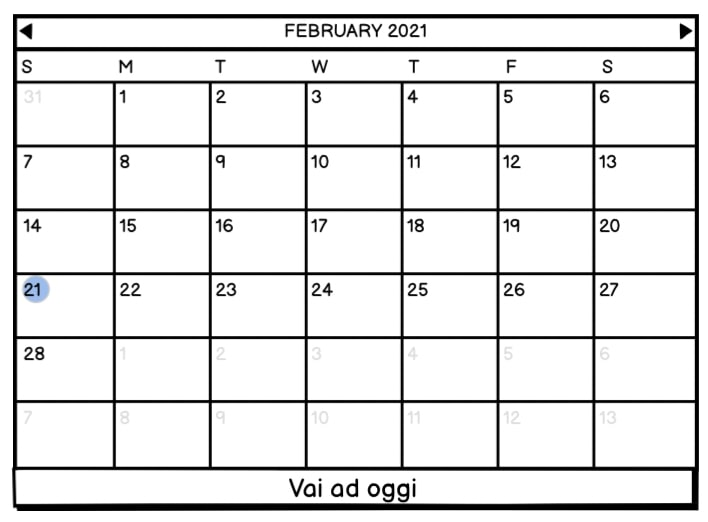
\includegraphics[width=0.5\textwidth]{wireframes/header-data-singola}
        \caption{Widget per selezionare una data singola.}\label{fig:header-data-singola}
    \end{subfigure}
\hfill
    \begin{subfigure}[b]{0.5\textwidth}
        \centering
        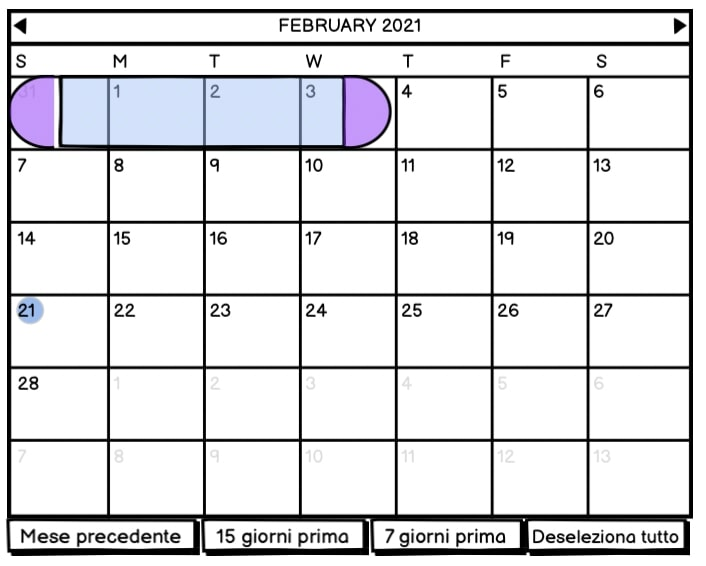
\includegraphics[width=0.5\textwidth]{wireframes/header-data-range}
        \caption{Widget per selezionare un range di date.}\label{fig:header-data-range}
    \end{subfigure}
    \caption{Widget per selzionare la data.}
\end{figure}

\begin{figure}[H]
    \centering
    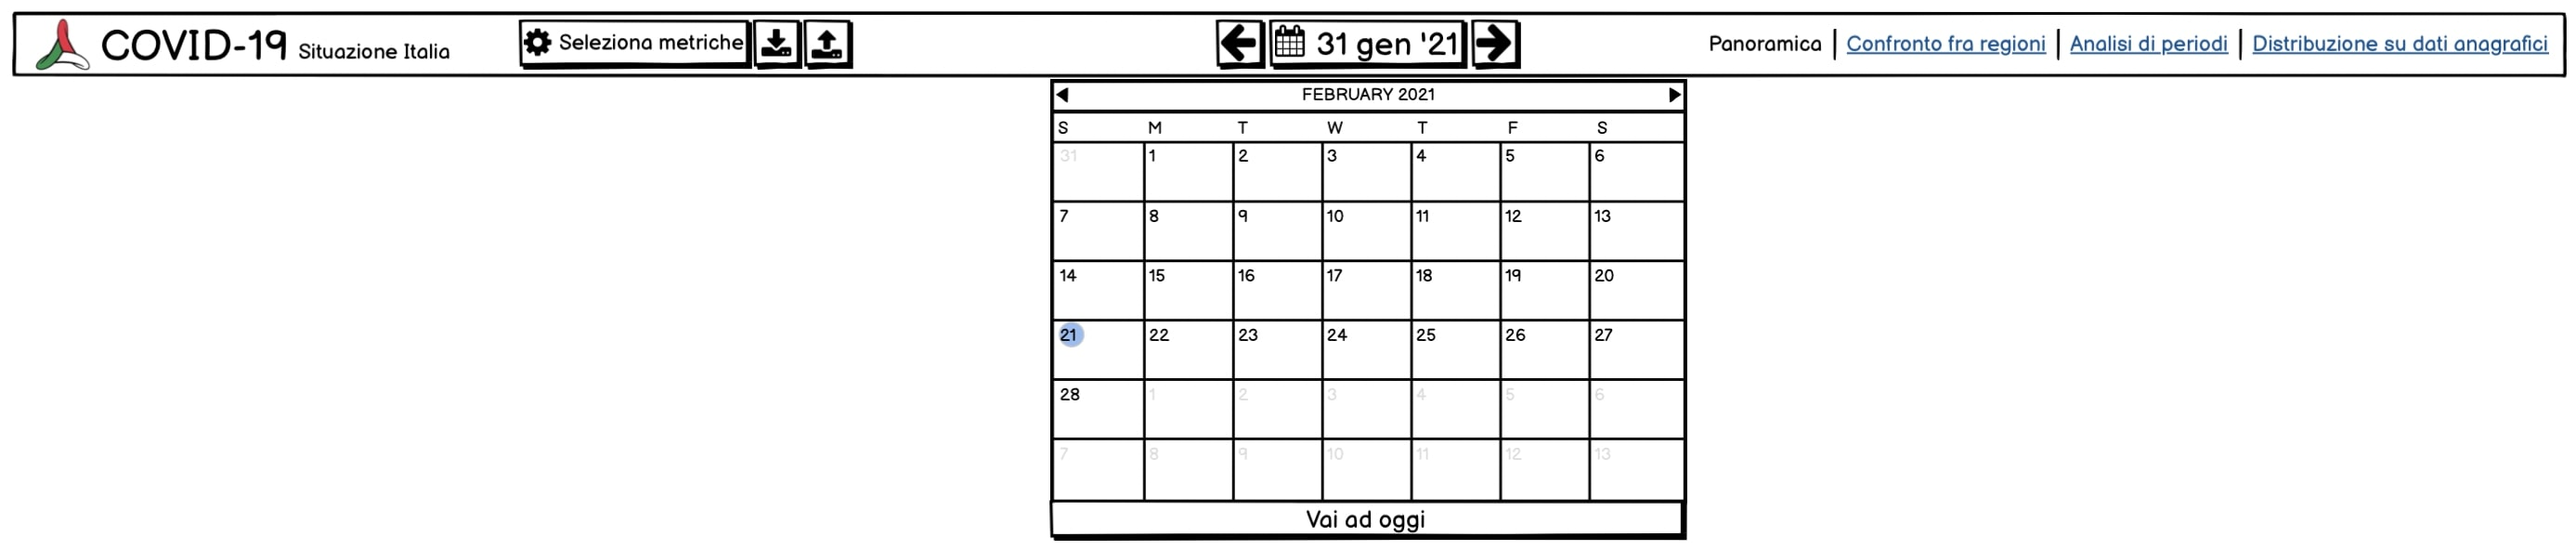
\includegraphics[width=1\columnwidth]{wireframes/header-data-aperta}
    \caption{Header con data aperta.}\label{fig:header-data-aperta}
\end{figure}

Nel widget per selezionare una data singola (\ref{fig:header-data-singola}) vi è un bottone per tornare rapidamente alla data odierna.\\
Nel widget per selezionare un range di date (\ref{fig:header-data-range}) vi sono diversi bottoni che permettono di velocizzare alcune operazioni come: andare al mese precedente, ai quindici giorni precedenti, ai sette giorni precedenti e per deselezionare il range.\\
In~\ref{fig:header-data-aperta} vi è una dimostrazione di come il widget appare rispetto all'header.

\begin{bclogo}{Selettore date}
    Inizialmente avevamo usato un semplice selettore di date (\ref{fig:selettore-data-singola-vecchia}); solo successivamente lo abbiamo arricchito di funzionalità quali attivabili mediante i pulsanti sotto il calendario.
\begin{figure}[H]
    \centering
    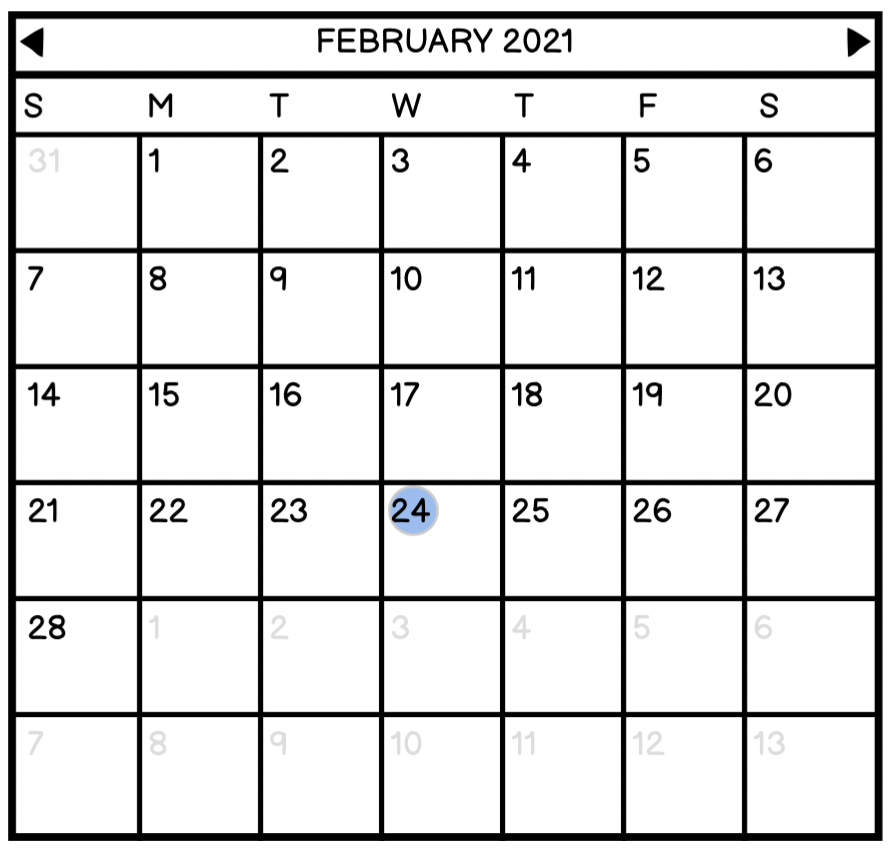
\includegraphics[width=0.3\columnwidth]{wireframes/selettore-data-singola-vecchia}
    \caption{Prima versione del selettore di date.}\label{fig:selettore-data-singola-vecchia}
\end{figure}
\end{bclogo}

\begin{figure}[H]
    \centering
    
\includegraphics[width=1\columnwidth]{wireframes/footer}
    \caption{Footer comune a tutte le schermate}\label{fig:footer}
\end{figure}

Nel footer (\ref{fig:footer}) vi sono alcune informazioni e link per le pagine istituzionali e le fonti dai quali i dati sono stati recuperati; da destra ci sono:
\begin{itemize}
    \item logo della Repubblica Italiana;
    \item logo e nome della Protezione Civile;
    \item link alle fonti e data dell'ultimo aggiornamento;
    \item link ai siti istituzionali.
\end{itemize}

\begin{bclogo}{Footer}
    Le prime versioni del footer erano sprovviste della data dell'ultimo aggiornamento. Successivamente ci siamo resi conto che tale informazione era essenziale per i giornalisti per sapere se stavano osservando dati aggiornati o meno.
\begin{figure}[H]
    \centering
    
\includegraphics[width=1\columnwidth]{wireframes/footer-vecchio}
    \caption{Prima versione del footer.}\label{fig:footer-vecchio}
\end{figure}
\end{bclogo}


\subsubsection{Panoramica}\label{ss:panoramica}
\begin{figure}[H]
    \centering
    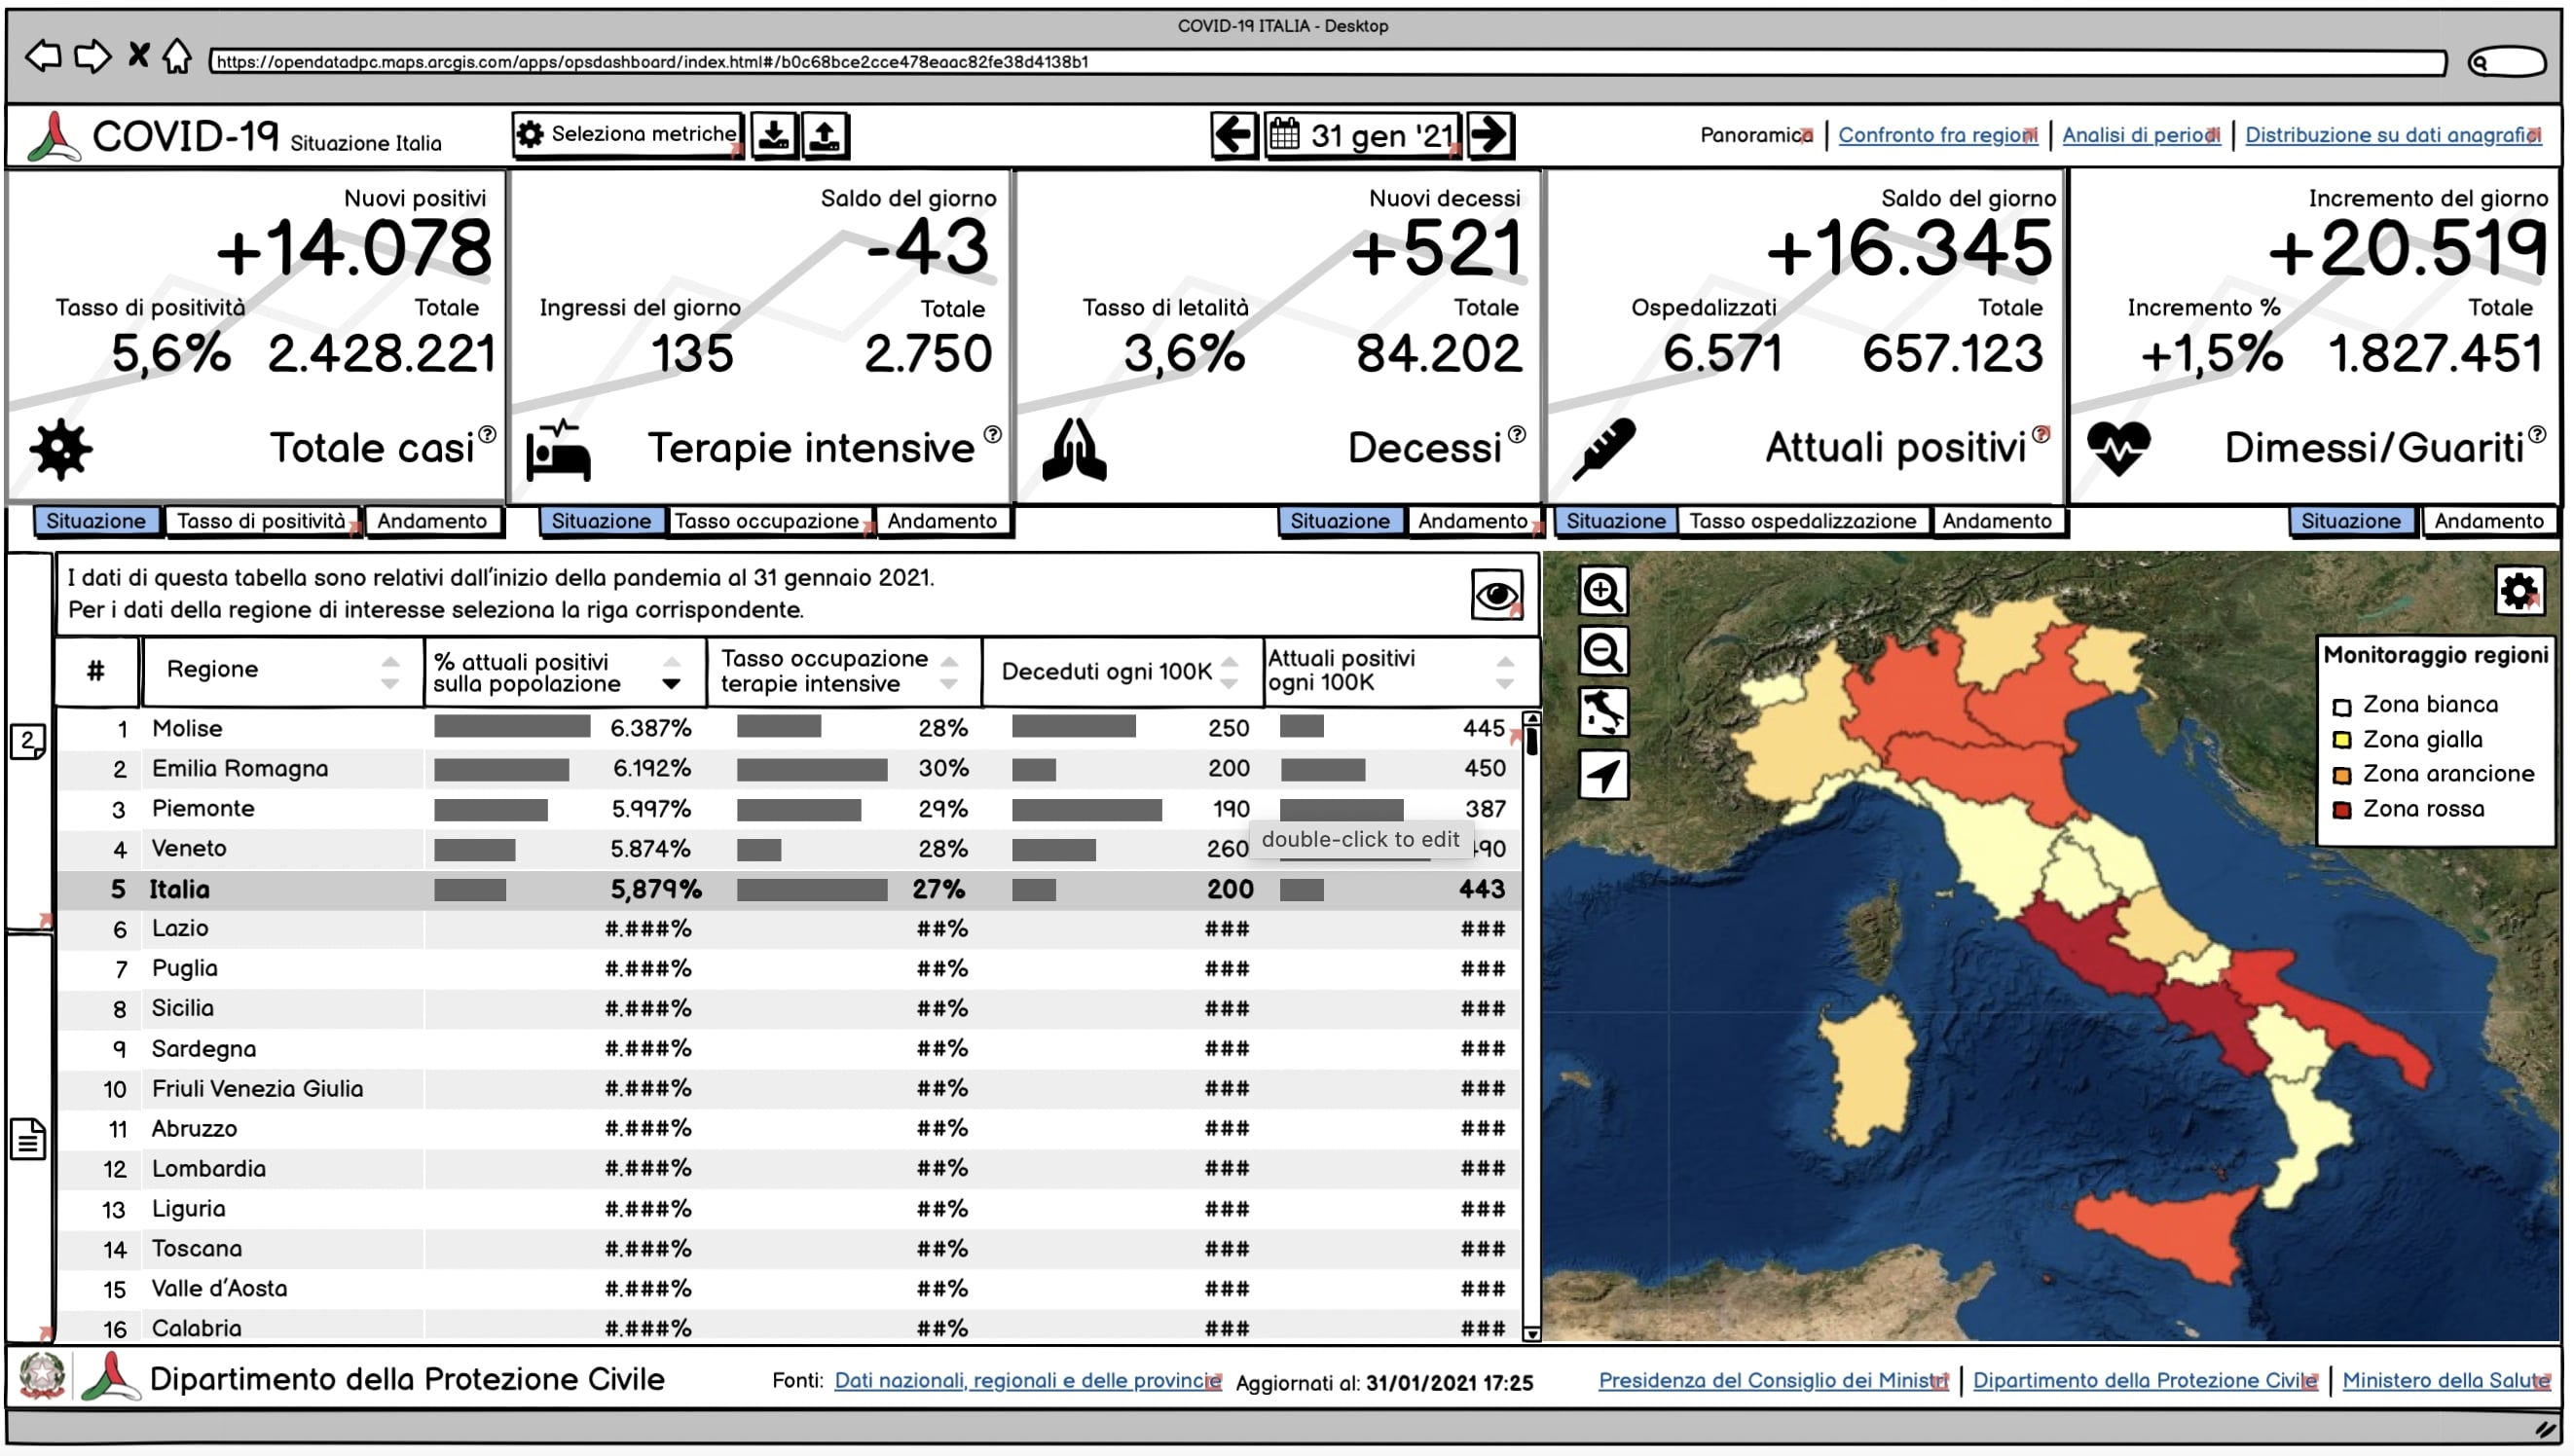
\includegraphics[width=1\columnwidth]{wireframes/panoramica}
    \caption{Schermata ``Panoramica''}\label{fig:panoramica}
\end{figure}
La schermata ``Panoramica'' è la prima schermata che un utente incontra aprendo la dashboard. \`E possibile dividere visivamente la schermata in due fasce: la fascia superiore che presenta cinque ``Box numerici'' e una fascia inferiore che presenta dei pulsanti per aprire le sidebar delle note e dei provvedimenti, una tabella e una \textit{heat map}.\\

\paragraph{Box numerici}
\begin{figure}[H]
    \centering
    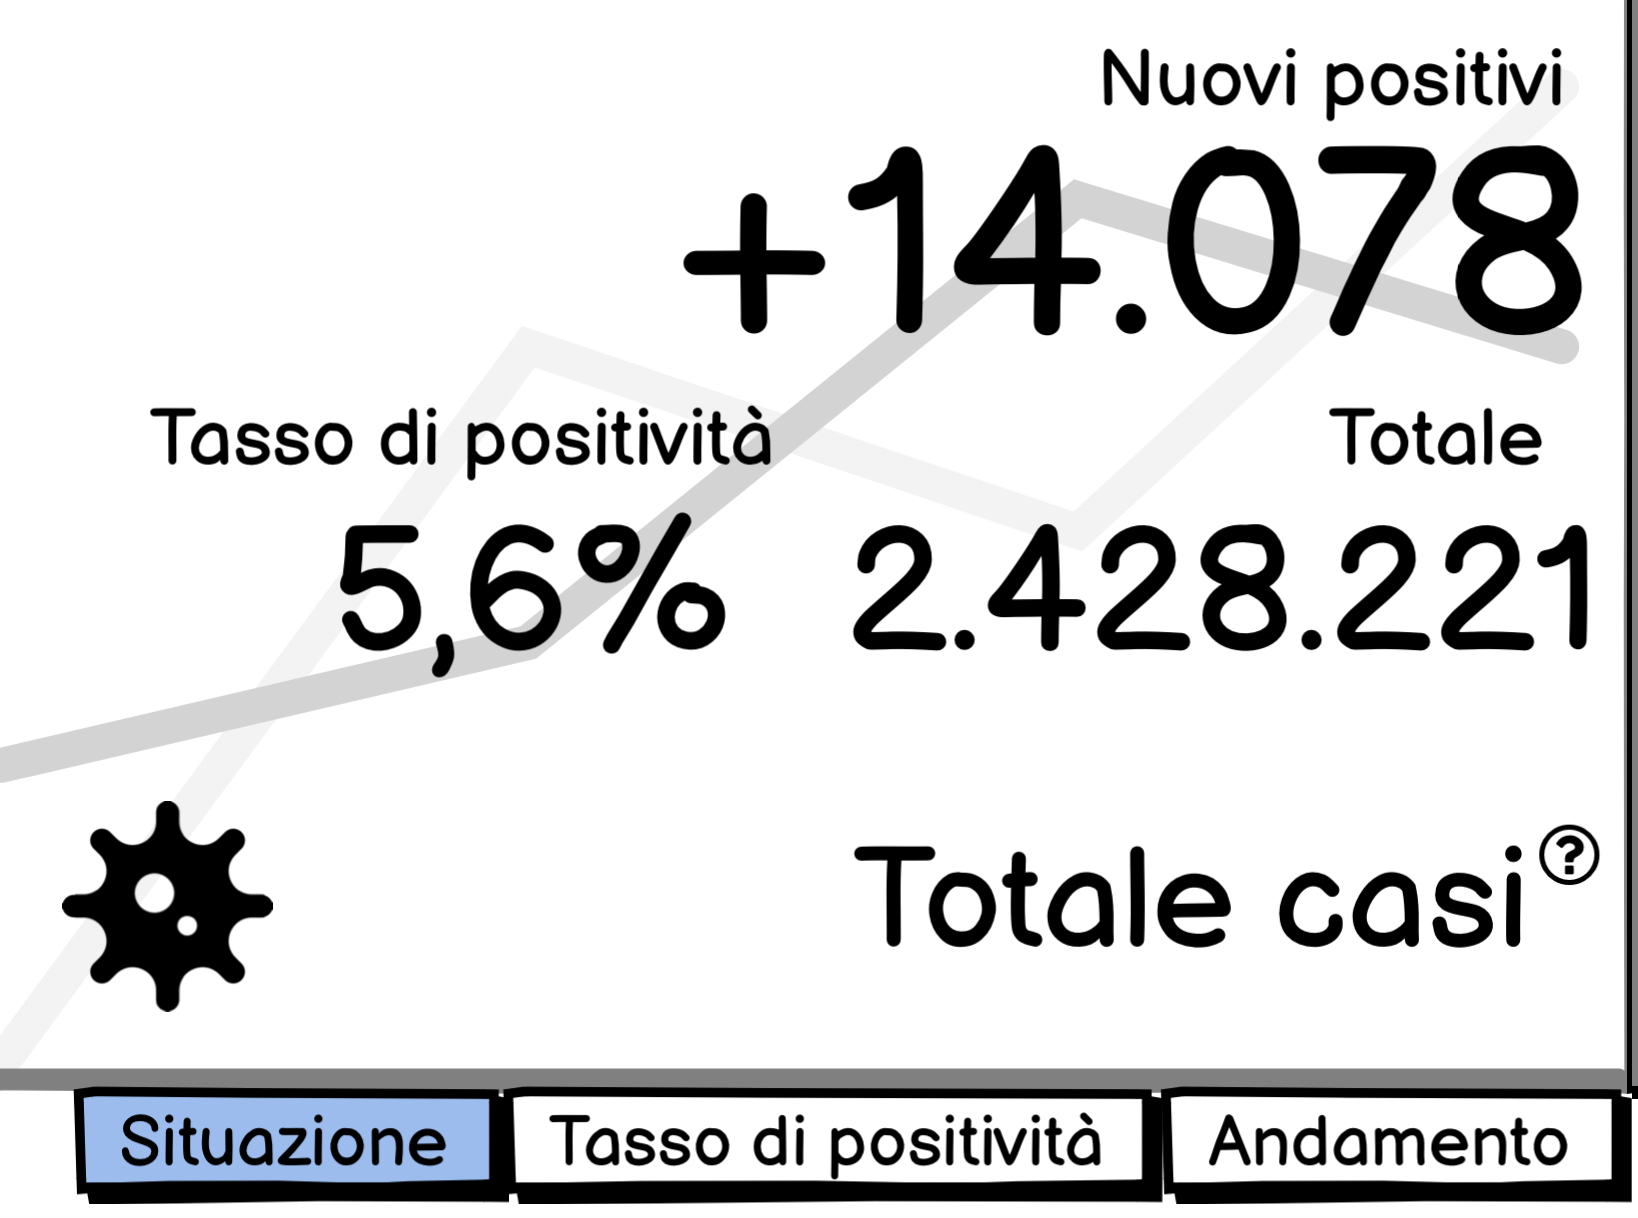
\includegraphics[width=0.5\columnwidth]{wireframes/box-numerico}
    \caption{Esempio di box numerico.}\label{fig:box-numerico}
\end{figure}

I cinque box numerici, di cui~\ref{fig:box-numerico} ne è un esempio, sono composti dal nome della metrica in basso e con una dimensione del font maggiore rispetto alle altre etichette, due tre valori numerici, ognuno dei quali ha al di sopra un'etichetta per spiegare a cosa quel valore si riferisce. Vi è inoltre un'icona, utile per aiutare la memoria e diminuire il carico cognitivo in quanto semplifica il riconoscimento del box. Come sfondo del box vi è la curva che rappresenta l'andamento della metrica.\\
Al di sotto di ogni box numerico vi sono due o tre pulsanti che cambiano il contenuto del box numerico: il pulsante ``Andamento'' mostra un grafico con l'andamento della metrica (\ref{fig:box-andamento}), il pulsante ``Tasso di \dots'' mostra una \textit{gauge} (\ref{fig:box-gauge}) mentre il pulsante ``Situazione'' mostra il box numerico mostrato di default all'apertura della pagina.

\begin{figure}[H]
    \begin{subfigure}[b]{0.5\textwidth}
        \centering
        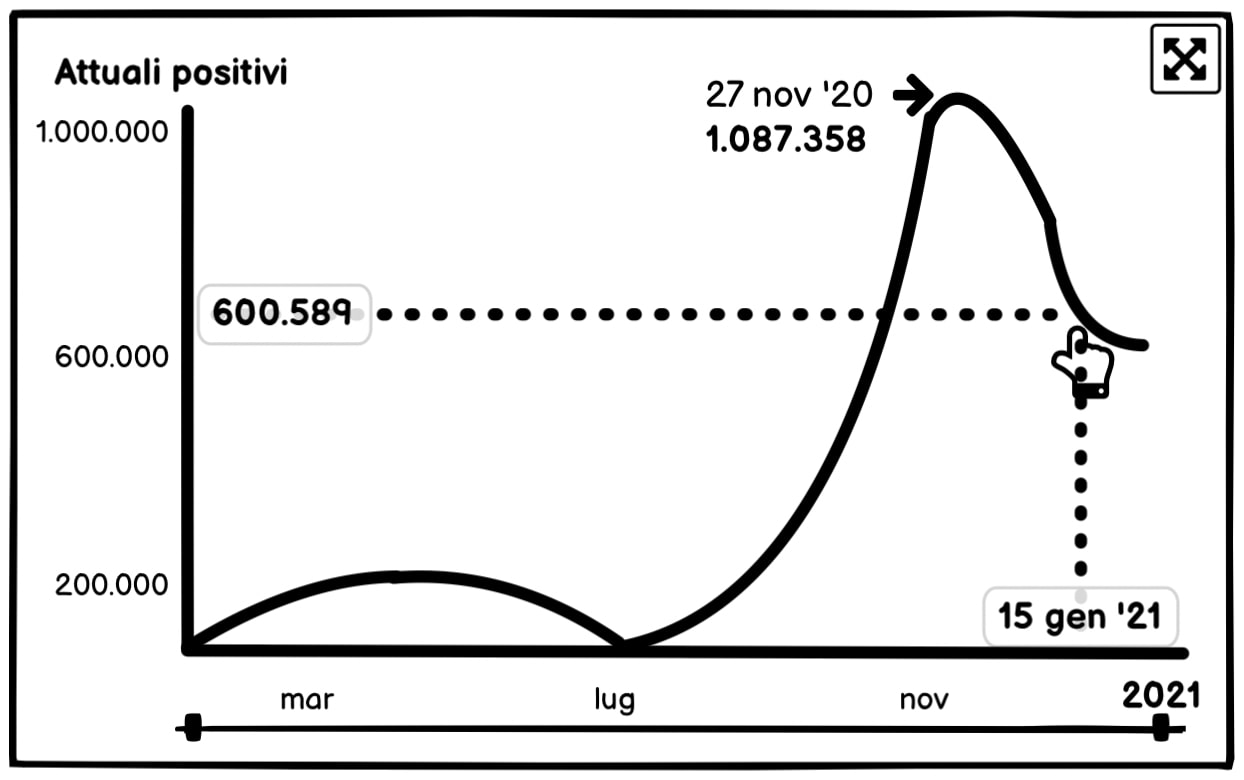
\includegraphics[width=1\textwidth]{wireframes/box-andamento}
        \caption{Box con grafico dell'andamento.}\label{fig:box-andamento}
    \end{subfigure}
\hfill
    \begin{subfigure}[b]{0.5\textwidth}
        \centering
        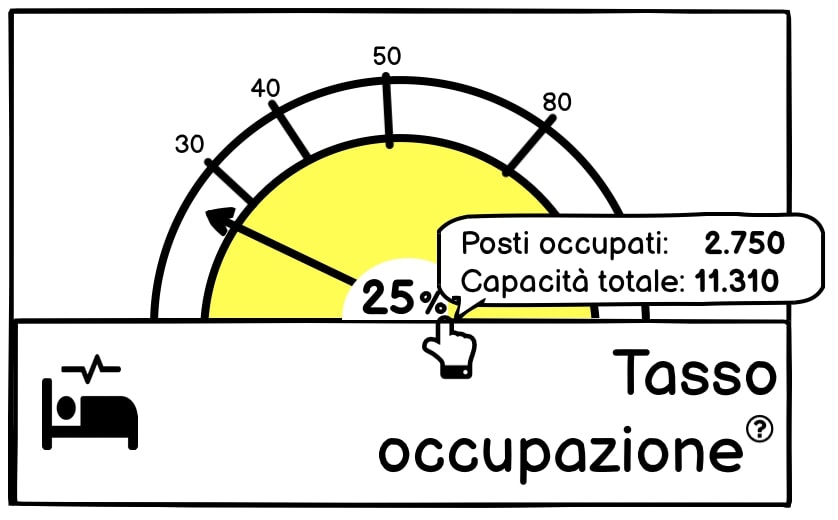
\includegraphics[width=1\textwidth]{wireframes/box-gauge}
        \caption{Box con gauge.}\label{fig:box-gauge}
    \end{subfigure}
    \caption{Viste alternative del ``Box numerico'' nella schermata ``Panoramica''.}
\end{figure}

\paragraph{Box con andamento}
I box con andamento possono avere due tipi di grafico in baso alla metrica rispetto alla quale si vuole osservare l'andamento: uno con una curva monotona crescente, utilizzato per mostrate l'andamento di metriche che possono solo salire (\ref{fig:box-andamento-monotono}) e un altro con una curva che non presenta monotonia (\ref{fig:box-andamento-no-monotonia}). 
\begin{figure}[H]
    \begin{subfigure}[b]{0.5\textwidth}
        \centering
        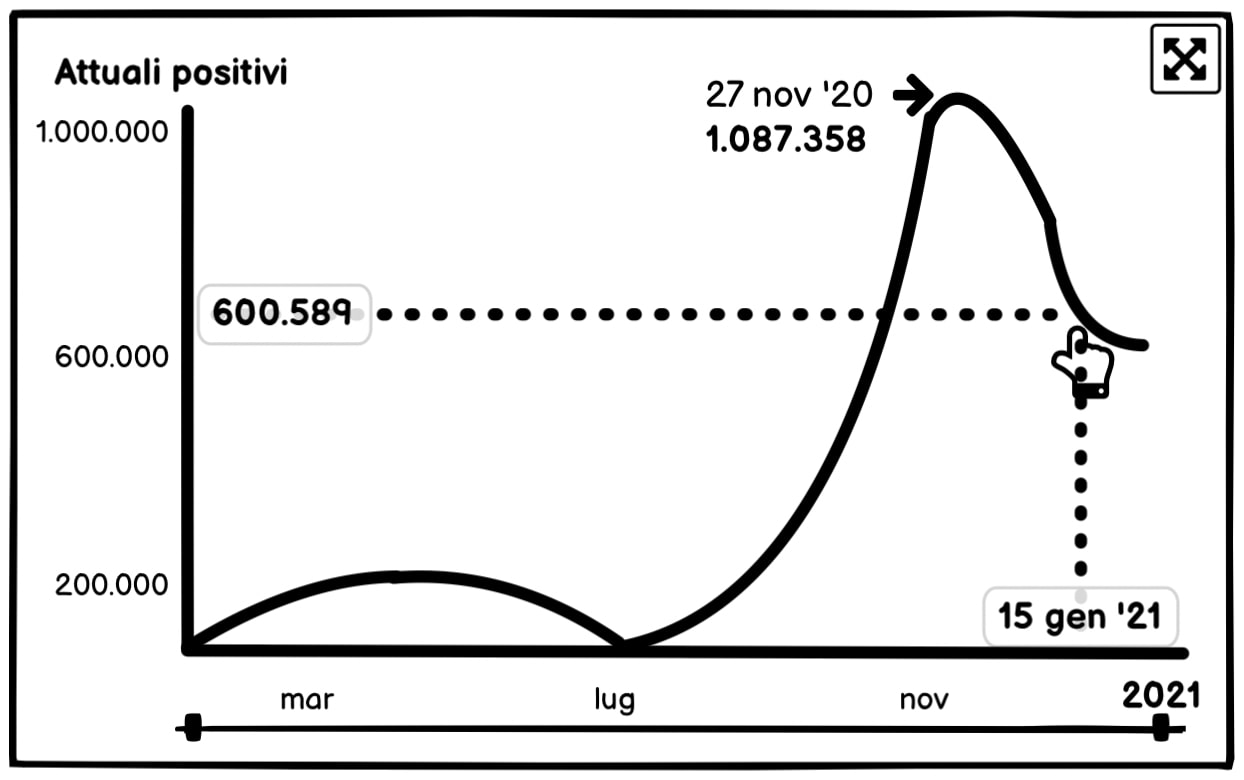
\includegraphics[width=1\textwidth]{wireframes/box-andamento}
        \caption{Box con grafico dell'andamento con una curva che non presenta monotonia.}\label{fig:box-andamento-no-monotonia}
    \end{subfigure}
\hfill
    \begin{subfigure}[b]{0.5\textwidth}
        \centering
        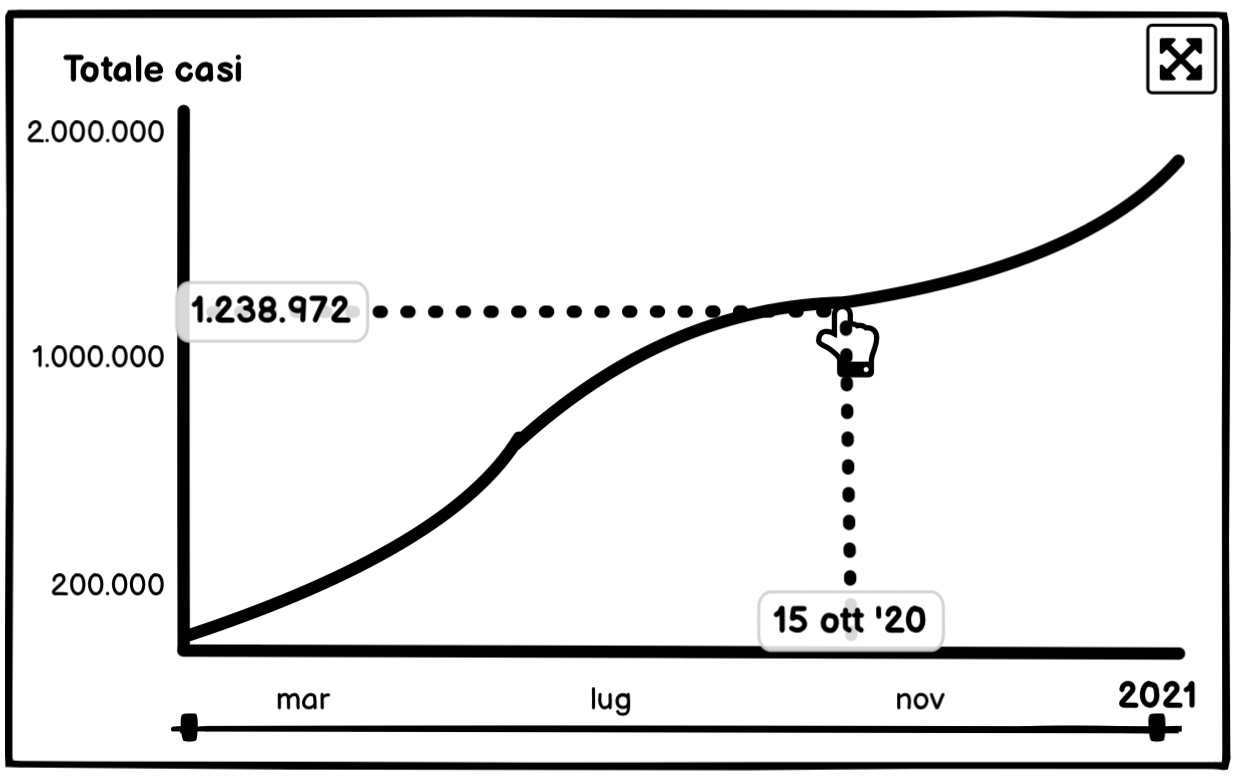
\includegraphics[width=1\textwidth]{wireframes/box-andamento-monotono}
        \caption{Box con grafico dell'andamento con una curva monotona crescente.}\label{fig:box-andamento-monotono}
    \end{subfigure}
    \caption{Differenti tipi di grafico dell'andamento di una metrica.}
\end{figure}

In~\ref{fig:box-andamento-no-monotonia} è presente un indicatore al valore massimo raggiunto, che, a differenza, in~\ref{fig:box-andamento-monotono} non è presente.\\
Comune a entrambi in grafici vi è uno slider vicino all'asse delle X con duplice selettore; questo slider può essere utilizzato per restringere il range di date che il grafico rappresenta. Inoltre in caso si passi sopra al grafico con il cursore, compare un tooltip che indica con precisione i valori raggiunti il giorno indicato dalla proiezione sull'asse delle X.\\
In questi grafici è presente un pulsante in alto a destra che permette di visualizzare il grafico a pieno schermo, un esempio di come la schermata cambia lo si può vedere in~\ref{fig:grafico-full-screen}. Lo stesso pulsante può essere utilizzato per far tornare il grafico alla sua dimensione originaria.
\begin{figure}[H]
    \centering
    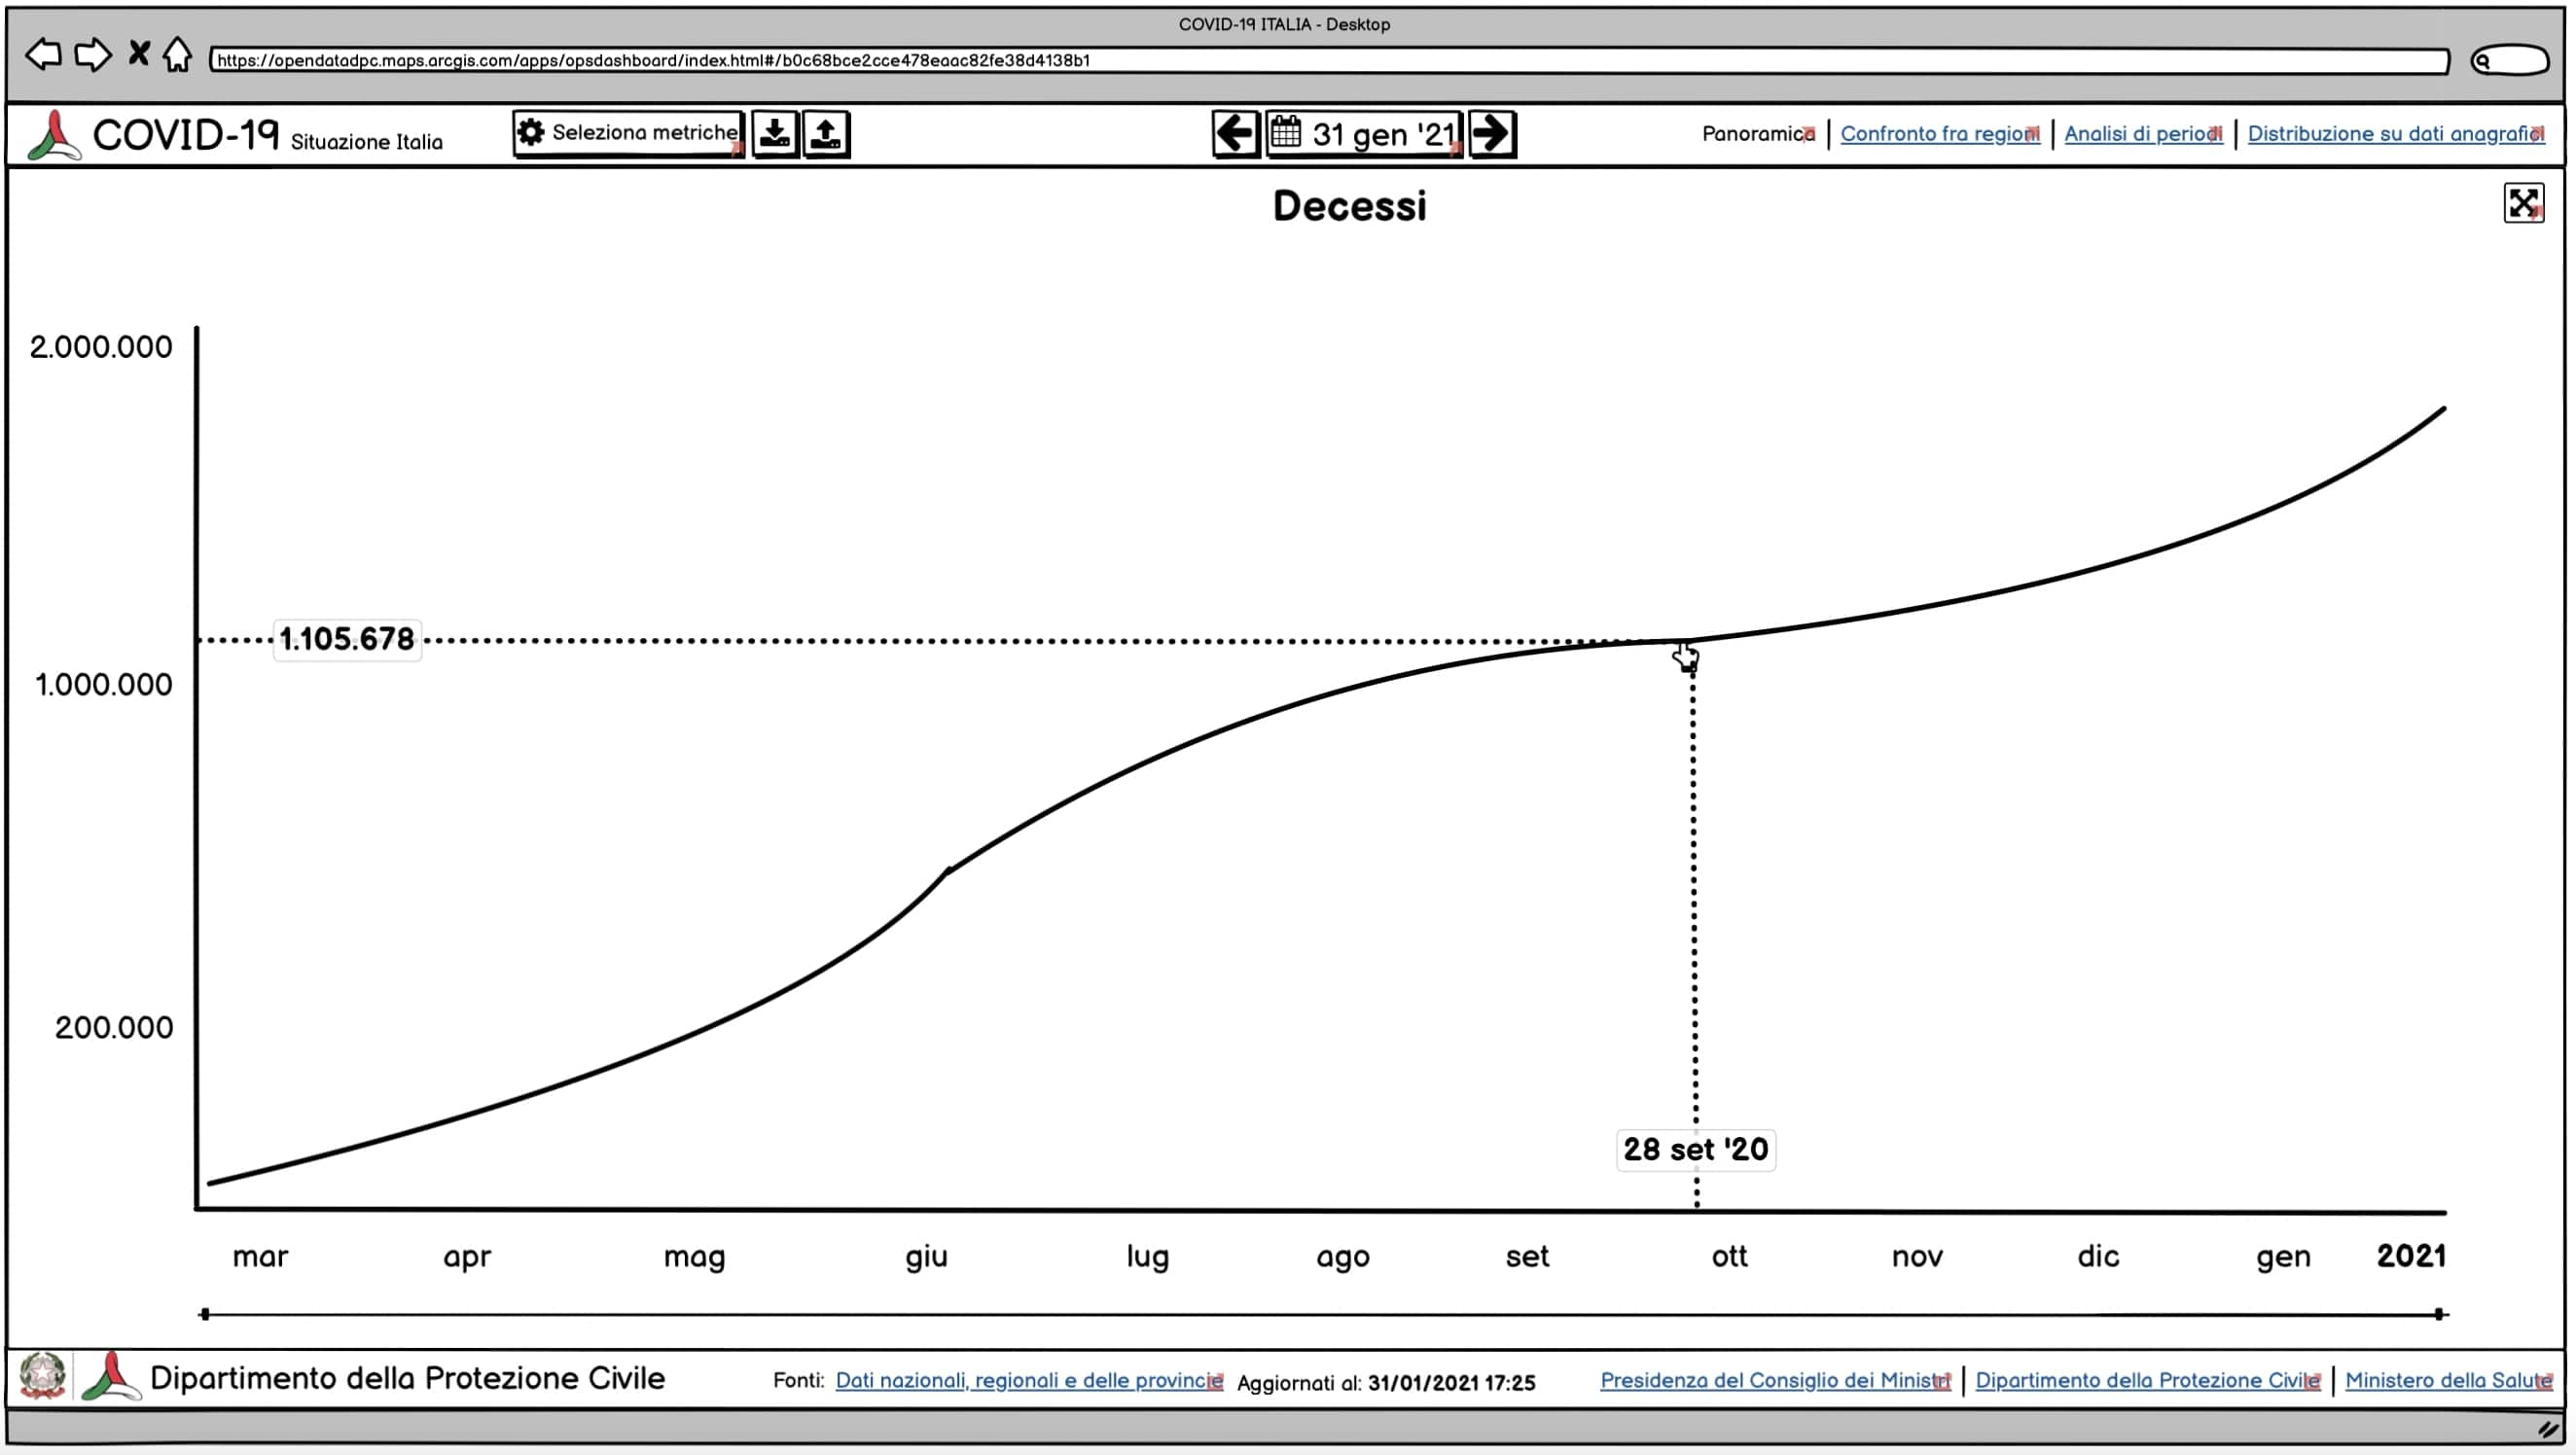
\includegraphics[width=0.7\columnwidth]{wireframes/grafico-full-screen}
    \caption{Grafico a pieno schermo}\label{fig:grafico-full-screen}
\end{figure}


\paragraph{Box con gauge}
I box con gauge sono utili per avere il colpo d'occhio di una specifica situazione (tasso di positività, tasso di occupazione delle terapie intensive, tasso di ospedalizzazioni). In caso si passi sopra alla gauge con il cursore, compare un tooltip che mostra i valori non percentuali di quella metrica.

\paragraph{Sidebar delle note e dei provvedimenti}
Sulla destra, vi sono due pulsanti che al click aprono due sidebar: una che mostra le note (\ref{fig:note}), ordinate cronologicamente e, l'altro, che mostra i provvedimenti (\ref{fig:provvedimenti}), anch'essi ordinati cronologicamente. 
\begin{figure}[H]
    \begin{subfigure}[b]{0.5\textwidth}
        \centering
        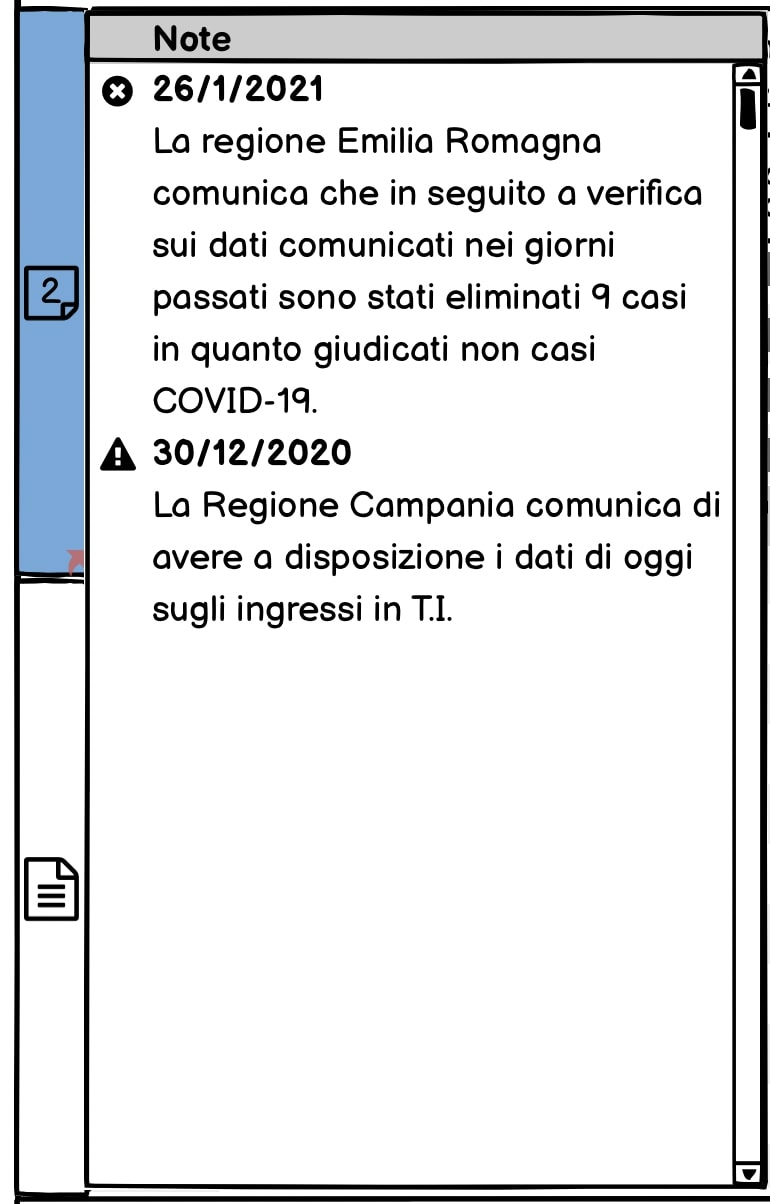
\includegraphics[width=1\textwidth]{wireframes/note}
        \caption{Sidebar delle note.}\label{fig:note}
    \end{subfigure}
\hfill
    \begin{subfigure}[b]{0.5\textwidth}
        \centering
        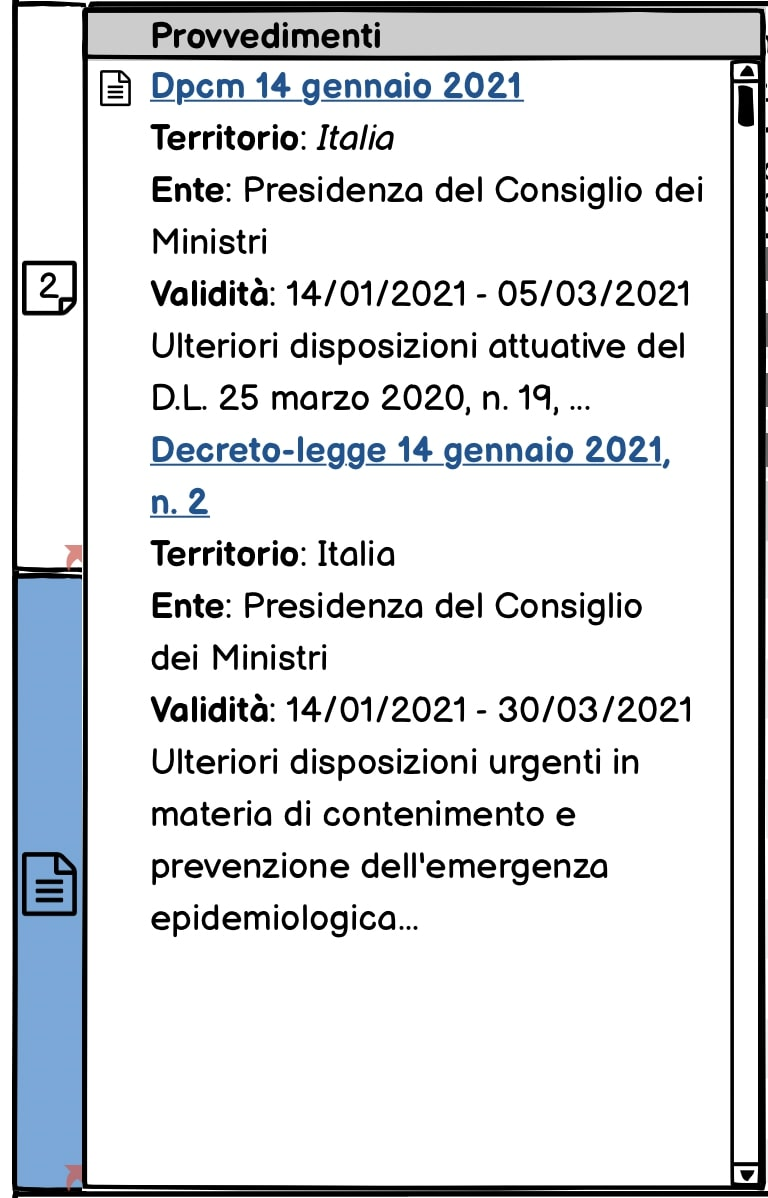
\includegraphics[width=1\textwidth]{wireframes/provvedimenti}
        \caption{Sidebar dei provvedimenti.}\label{fig:provvedimenti}
    \end{subfigure}
    \caption{Differenti tipi di grafico dell'andamento di una metrica.}
\end{figure}
In caso venga pubblicata una nuova nota o un nuovo provvedimento mentre si sta utilizzando la dashboard, l'utente viene notificato con la comparsa del numero di nuove note o nuovi provvedimenti sul pulsante; nel caso di~\ref{fig:note} abbiamo simulato la presenza di due nuove note.

\paragraph{Tabella}
\begin{figure}[H]
    \centering
    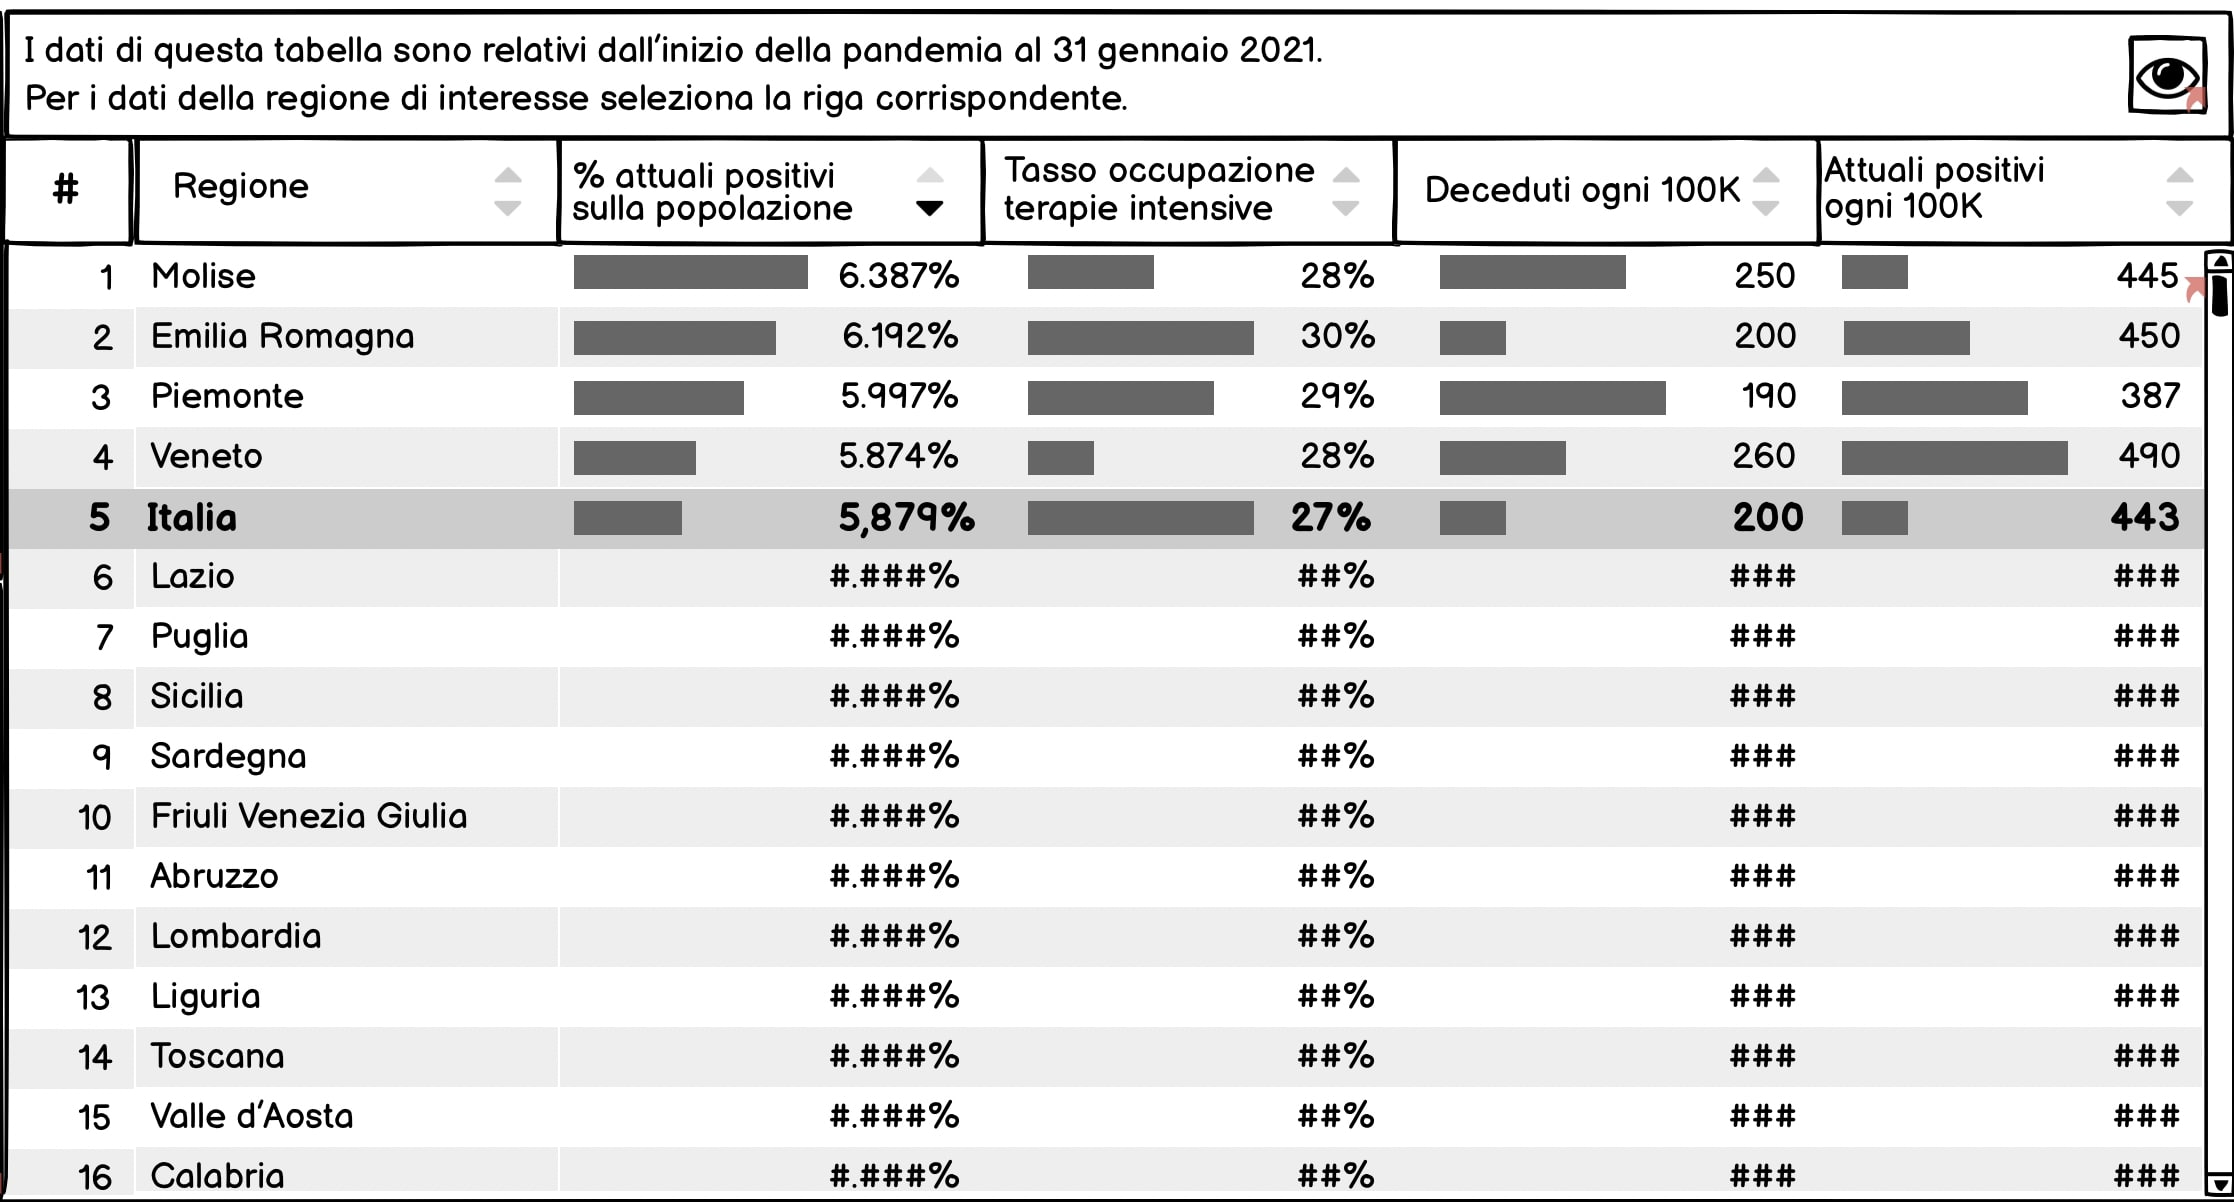
\includegraphics[width=0.7\columnwidth]{wireframes/tabella}
    \caption{Tabella delle regioni}\label{fig:tabella}
\end{figure}
Nella tabella in~\ref{fig:tabella} vi è l'elenco delle regioni italiane con associate alcune metriche. Le metriche visualizzate possono essere modificate cliccando sul pulsante con icona un occhio; il click apre una lista di metriche~\ref{fig:lista-metriche-tabella} che possono essere selezionate tramite una \textit{check-box}. Le colonne della tabella offrono la funzionalità di ordinamento per semplificare il confronto tra le diverse regioni, inoltre è presente una riga rappresentante la situazione dell'Italia in modo da permettere il confronto tra una regione e la media nazionale.\\
Cliccando su una regione i dati dell'intera schermata vengono aggiornati con i dati della regione cliccata, per esempio, cliccando sulla regione Molise si ottiene la schermata in~\ref{fig:panoramica-regione}. Nella tabella di questa vista sono presenti i dati riferiti alle province della regione selezionata assieme ai dati della regione e a quelli nazionali. Per tornare alla vista nazionale è possibile cliccare sulla riga dell' Italia nella tabella.
\begin{figure}[H]
    \centering
    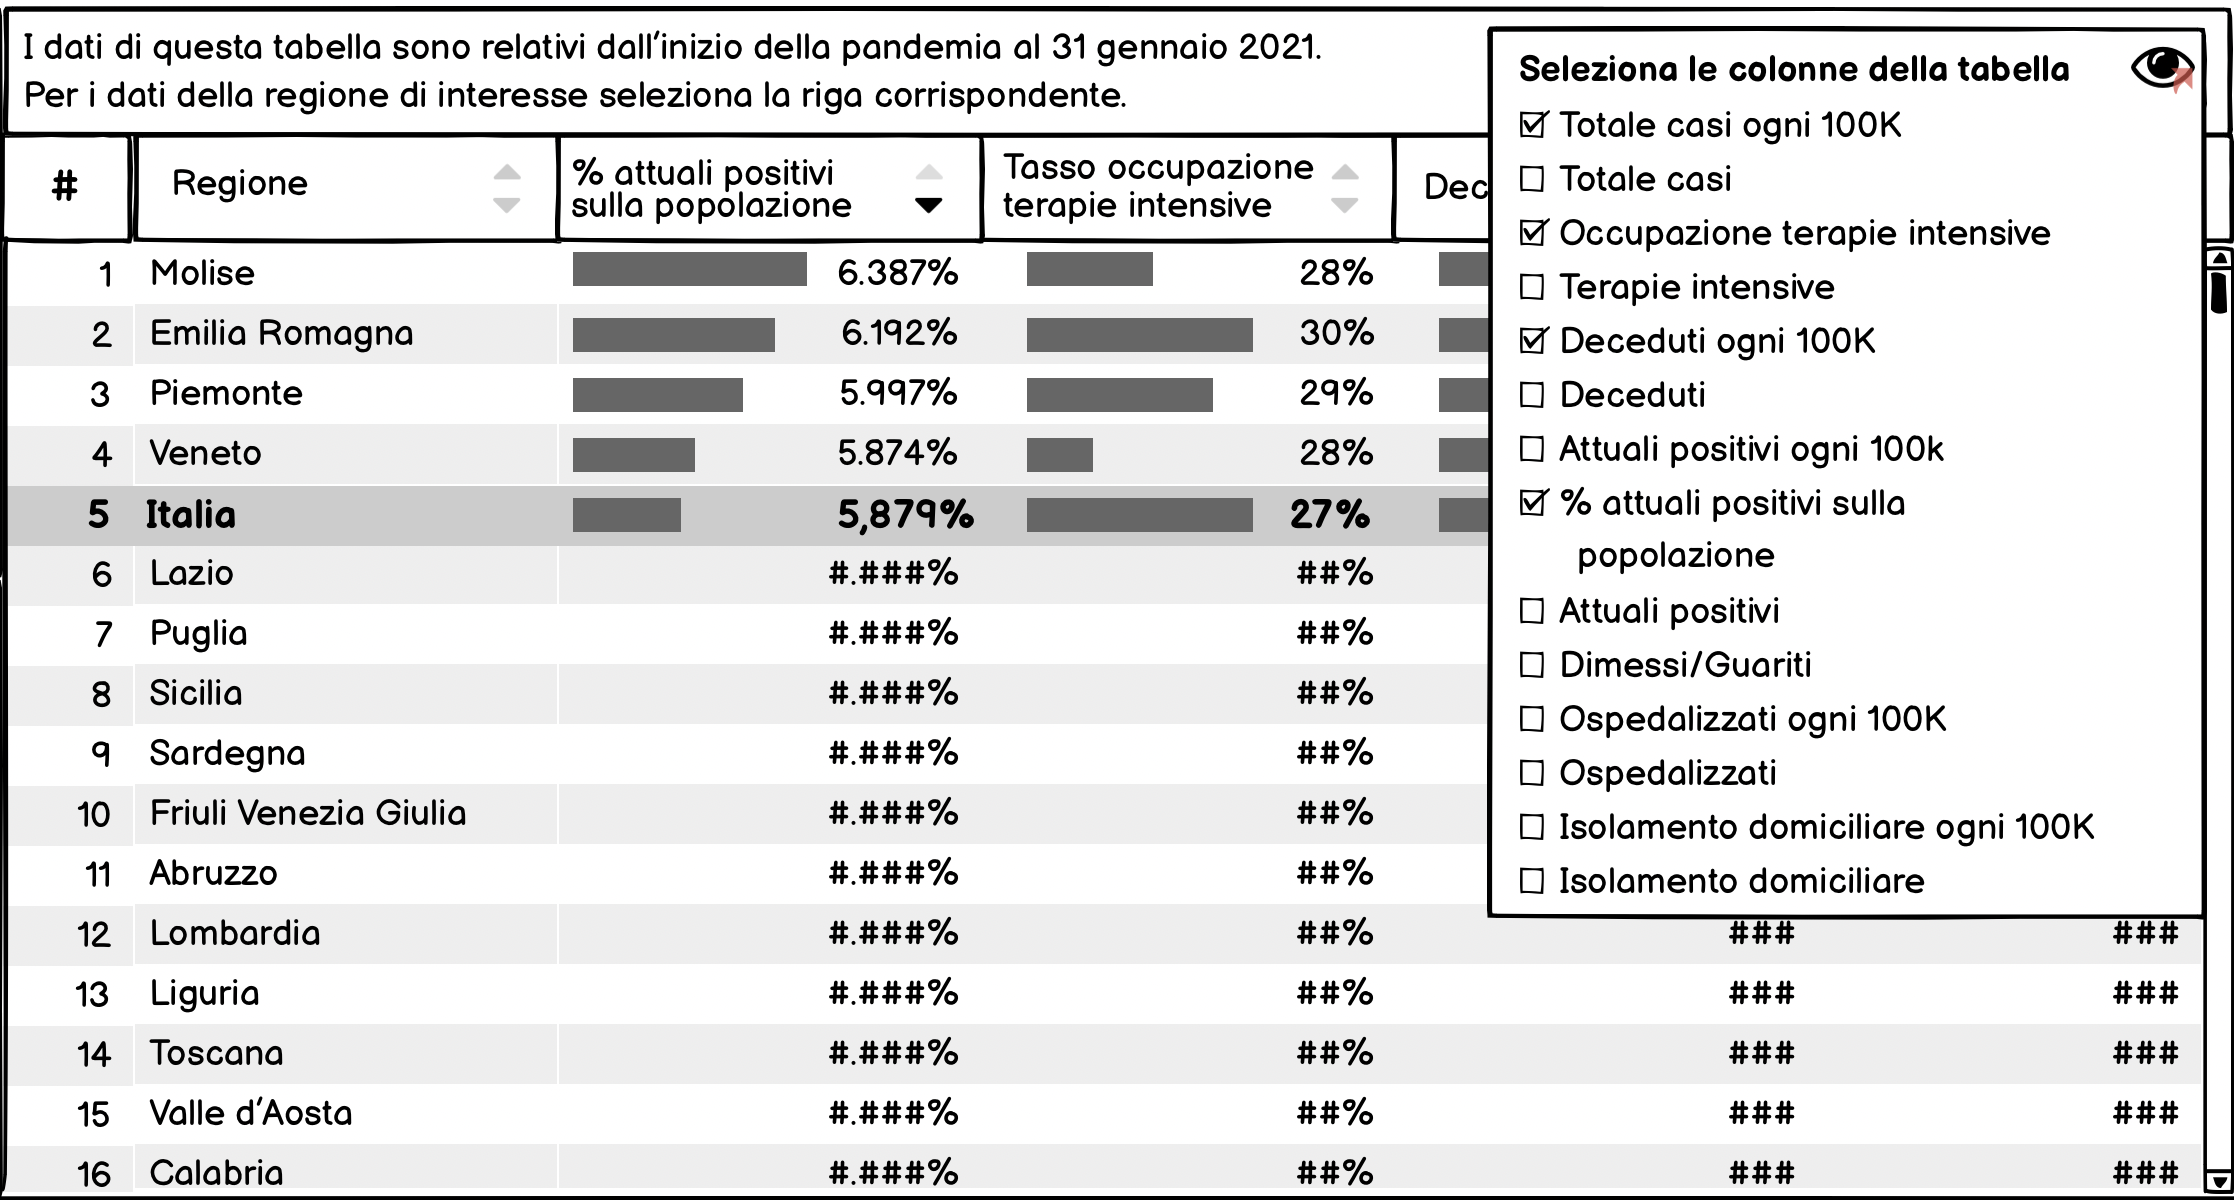
\includegraphics[width=0.7\columnwidth]{wireframes/lista-metriche-tabella}
    \caption{Lista delle metriche visionabili nella tabella.}\label{fig:lista-metriche-tabella}
\end{figure}

\begin{figure}[H]
    \centering
    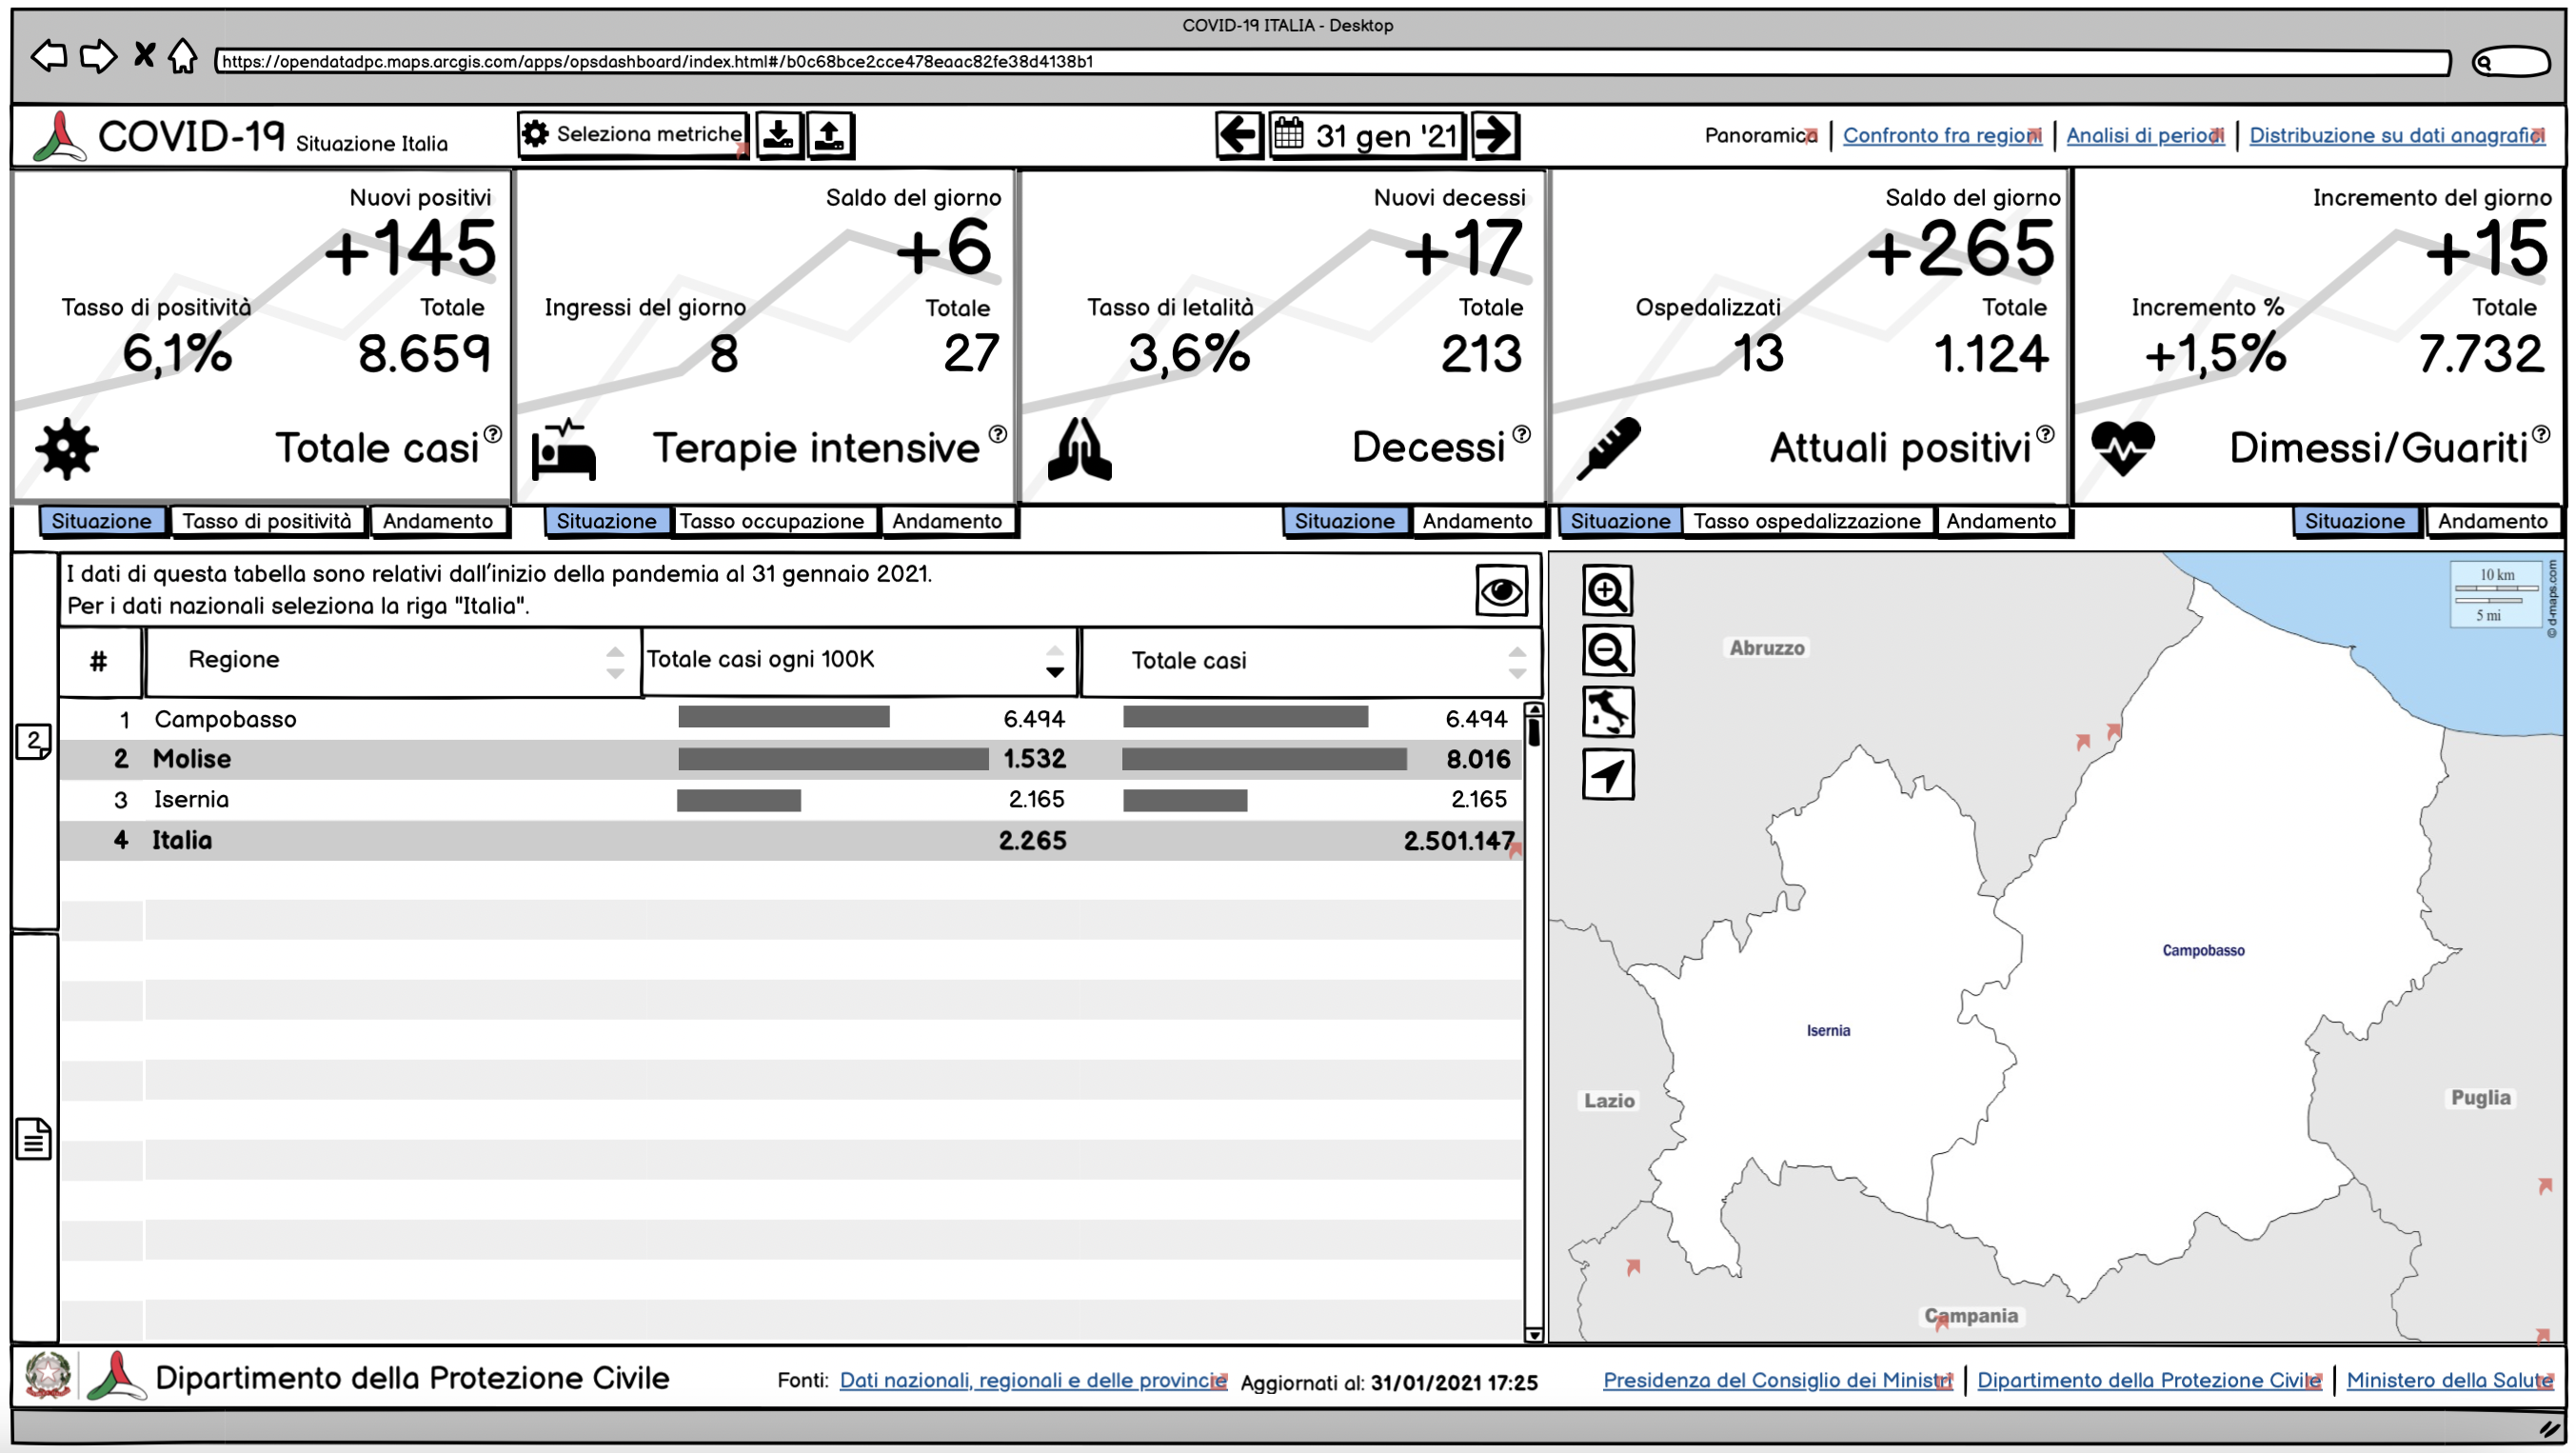
\includegraphics[width=0.7\columnwidth]{wireframes/panoramica-regione}
    \caption{Panoramica della regione Molise.}\label{fig:panoramica-regione}
\end{figure}

\paragraph{Mappa}
La mappa (\ref{fig:mappa-panoramica}) è uno strumento utile per avere un colpo d'occhio immediato sulla situazione dell'Italia o di una singola regione rispetto a una specifica metrica. Tale metrica è modificabile cliccando sulla ghiera in alto a destra; al click si apre una lista di metriche (\ref{fig:lista-metriche-mappa}) rispetto le quali è possibile studiare la mappa.
\begin{figure}[H]
    \centering
    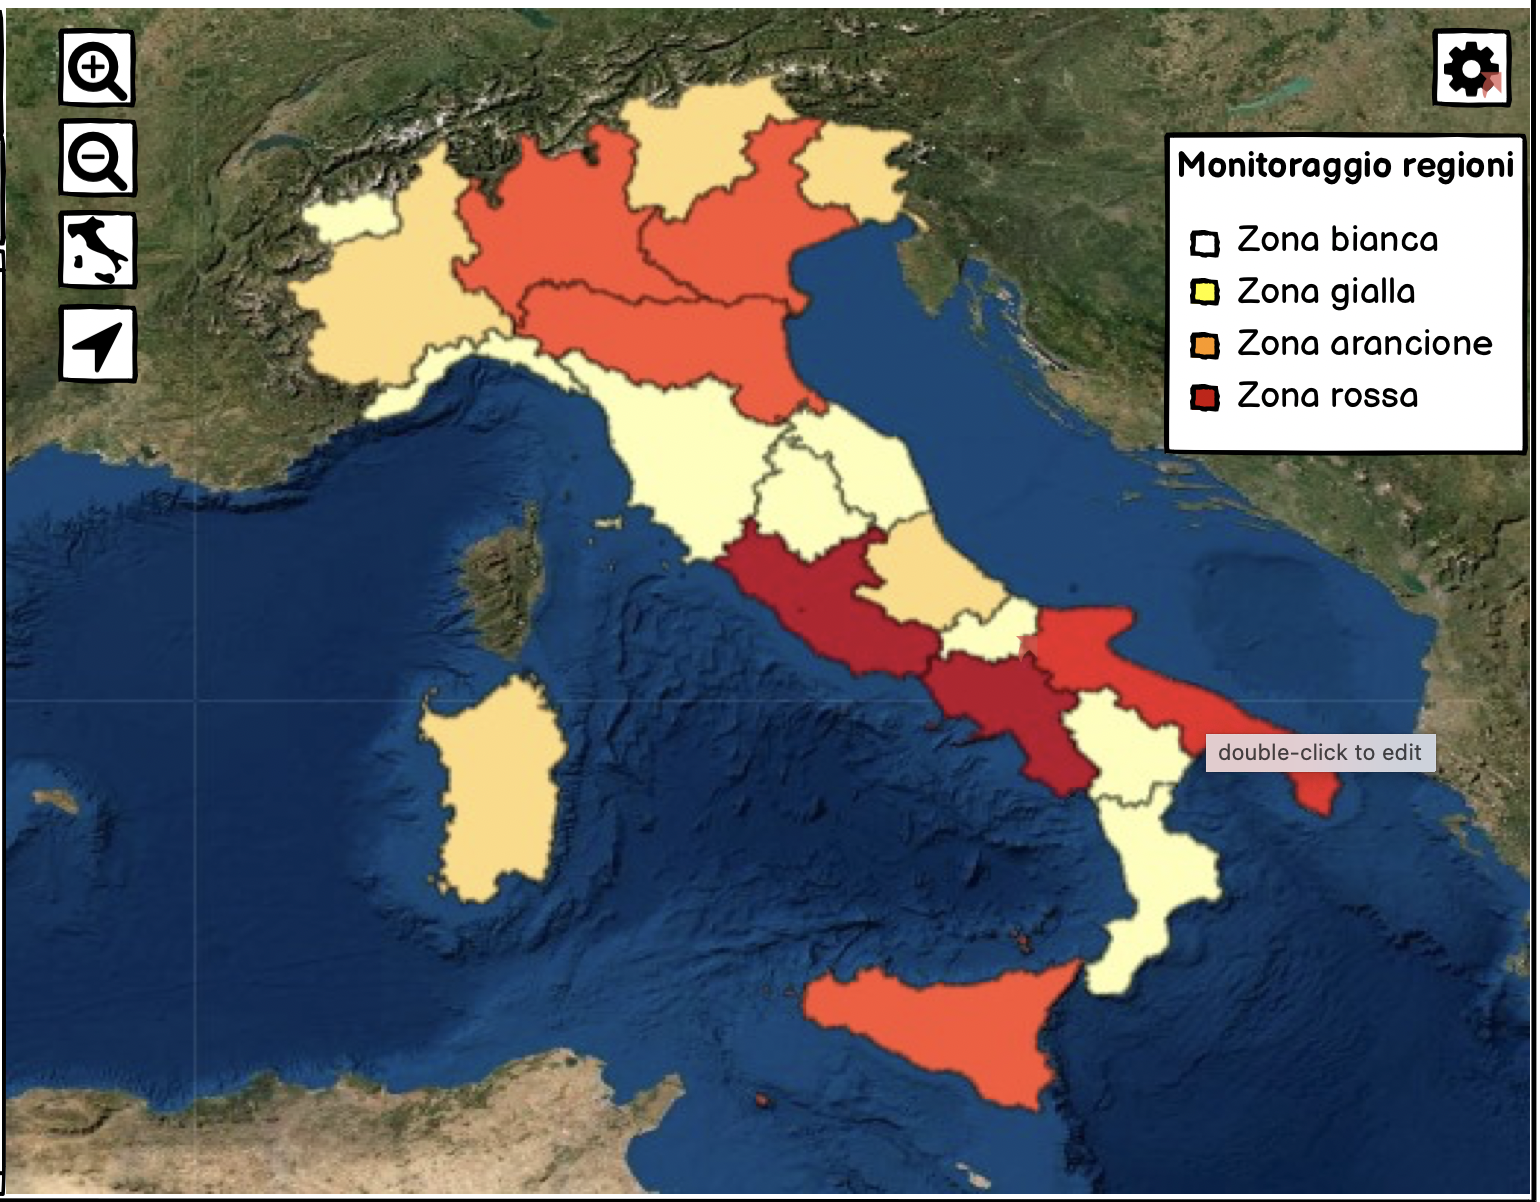
\includegraphics[width=0.7\columnwidth]{wireframes/mappa-panoramica}
    \caption{Heat map dell'Italia visualizzata nella scheda ``Panoramica''.}\label{fig:mappa-panoramica}
\end{figure}

\begin{figure}[H]
    \centering
    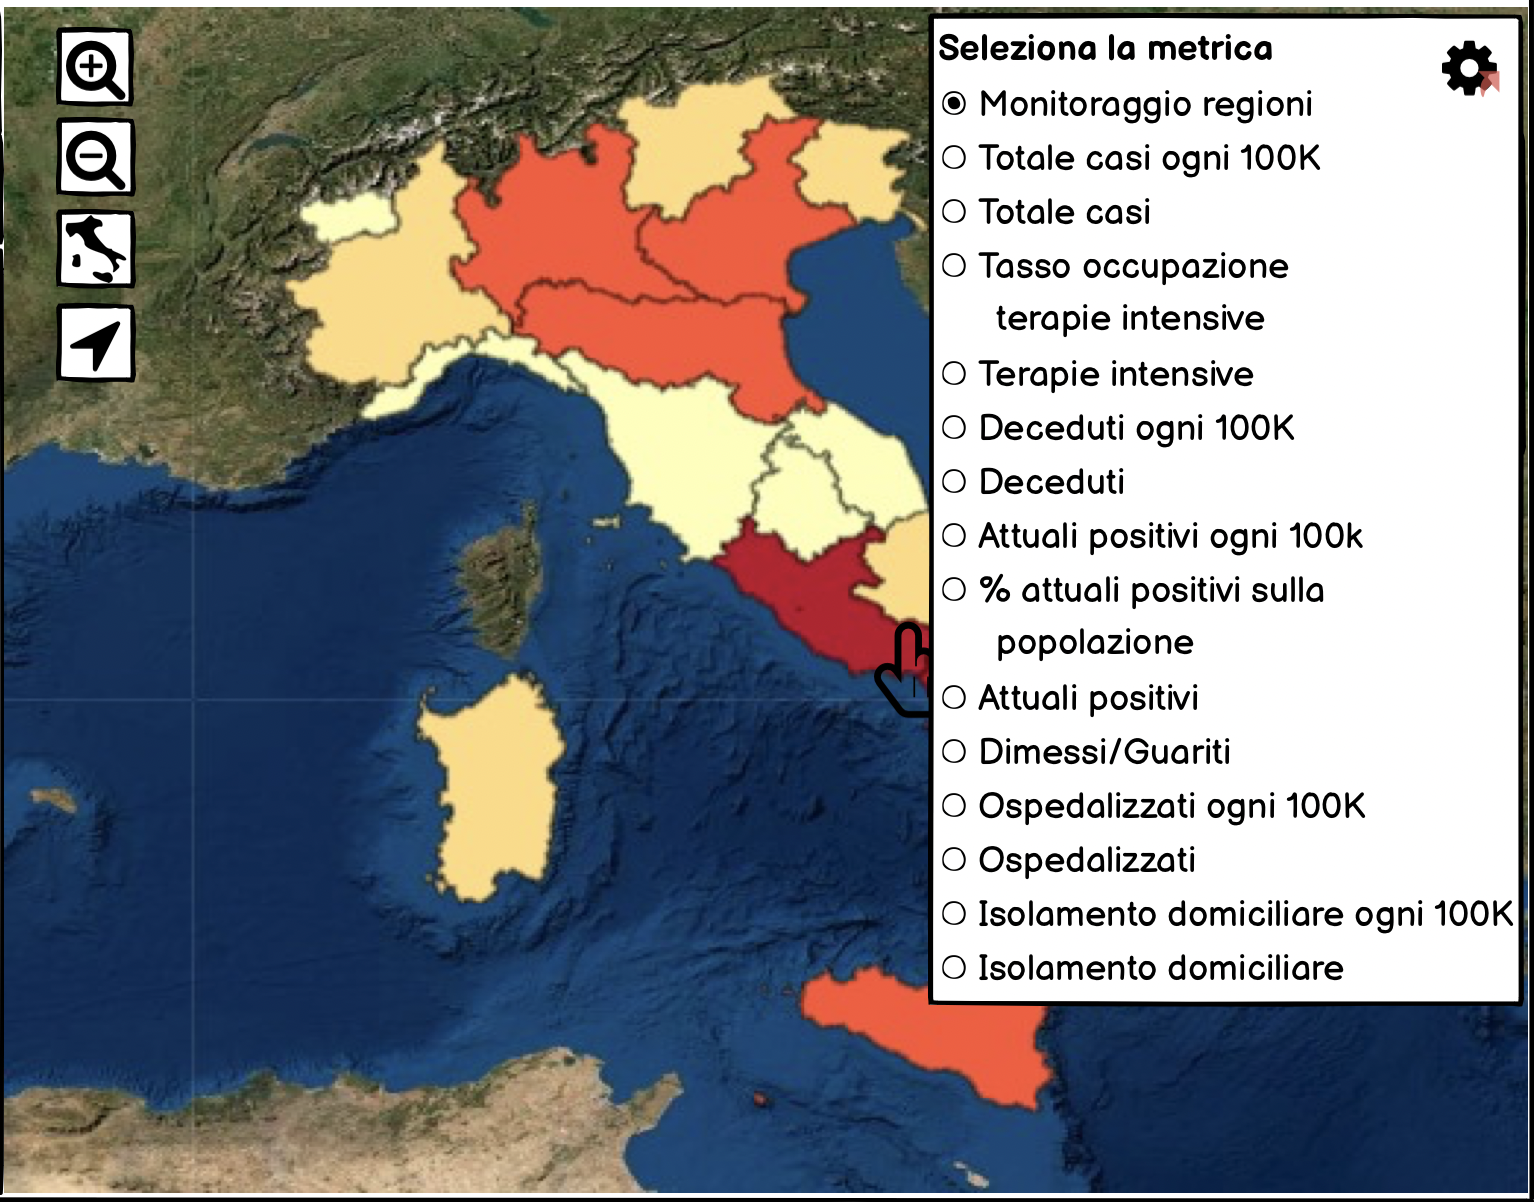
\includegraphics[width=0.7\columnwidth]{wireframes/lista-metriche-mappa}
    \caption{Lista delle metriche disponibili per la heat map.}\label{fig:lista-metriche-mappa}
\end{figure}

Cliccando su di una regione della tabella è inoltre possibile passare alla vista regionale della schermata ``Panoramica'' come in~\ref{fig:panoramica-regione}. Oltre a cliccare sulla riga dell'Italia nella tabella, per tornare alla panoramica nazionale è possibile anche cliccare al di fuori dei confini regionali nella mappa.

\paragraph{Caricamento dei dati}
Abbiamo previsto una schermata di caricamento in attesa che i dati vengano scaricati e computati prima di essere mostrati; abbiamo usato degli spinner per indicare ciò.
\begin{figure}[H]
    \centering
    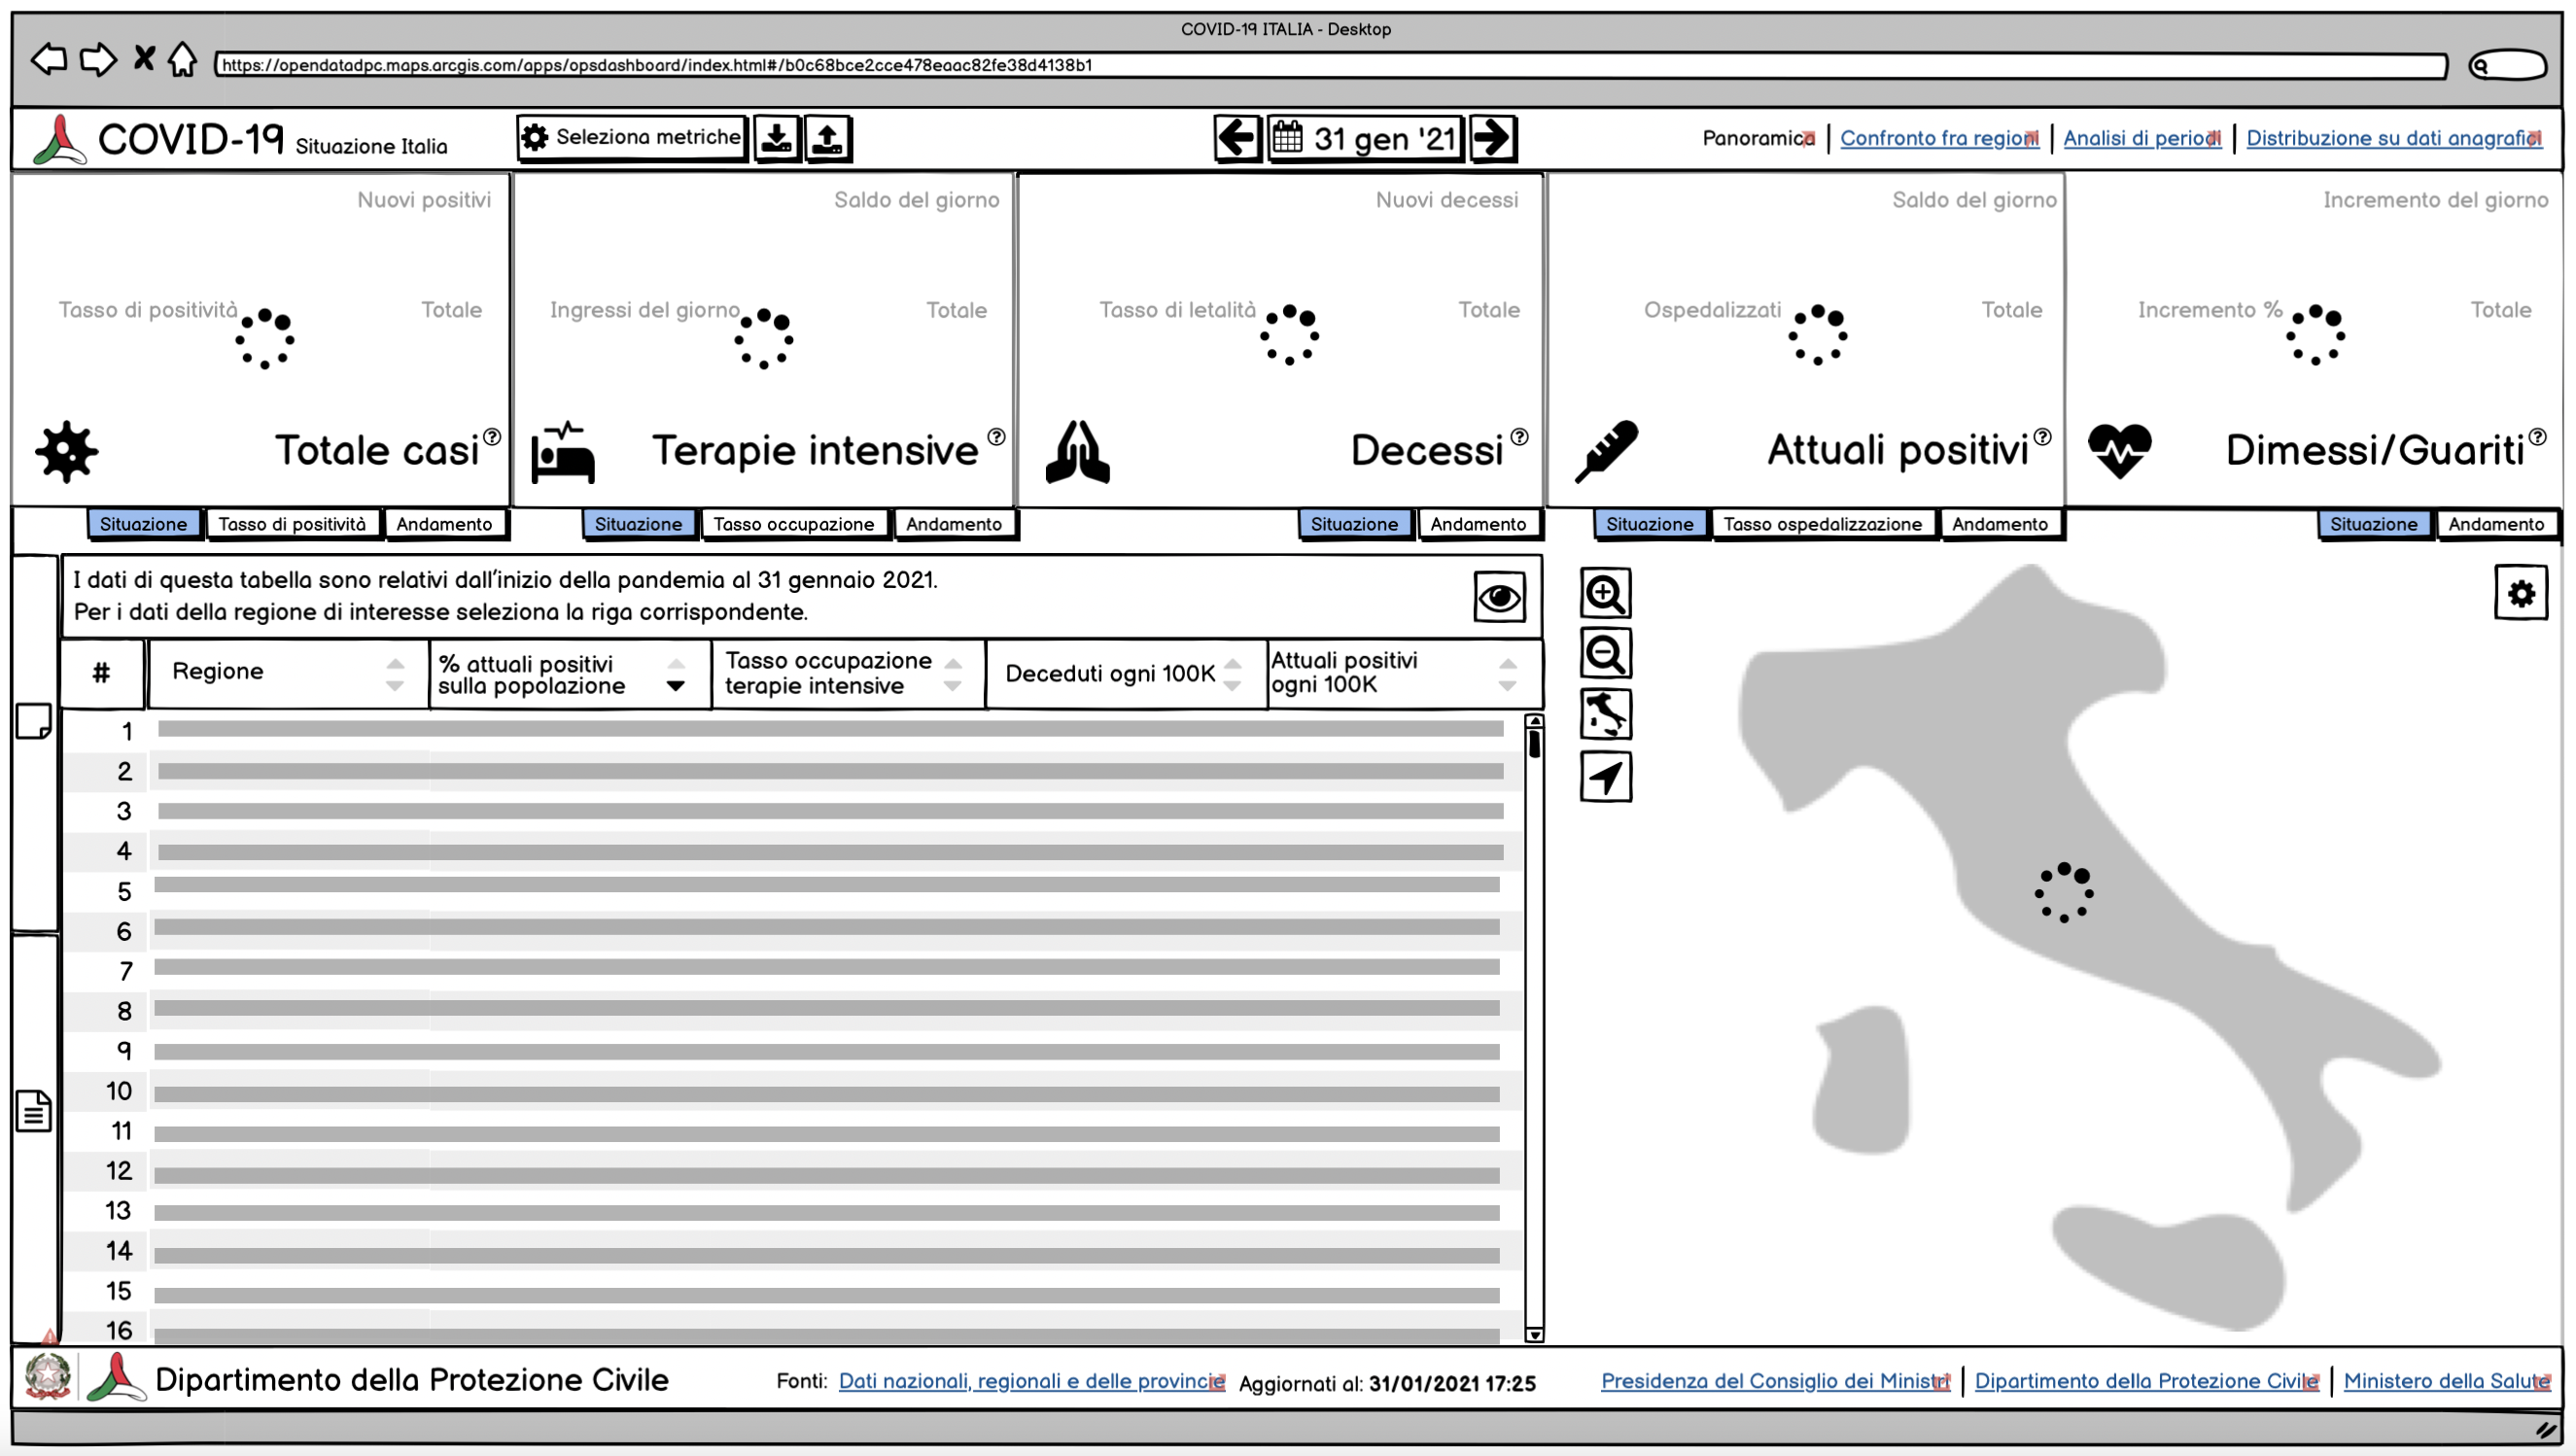
\includegraphics[width=1\columnwidth]{wireframes/panoramica-caricamento}
    \caption{Schermata ``Panoramica'' durante il caricamento dei dati.}\label{fig:panoramica-caricamento}
\end{figure}


\subsubsection{Confronto fra regioni}\label{ss:confronto-fra-regioni}
\begin{figure}[H]
    \centering
    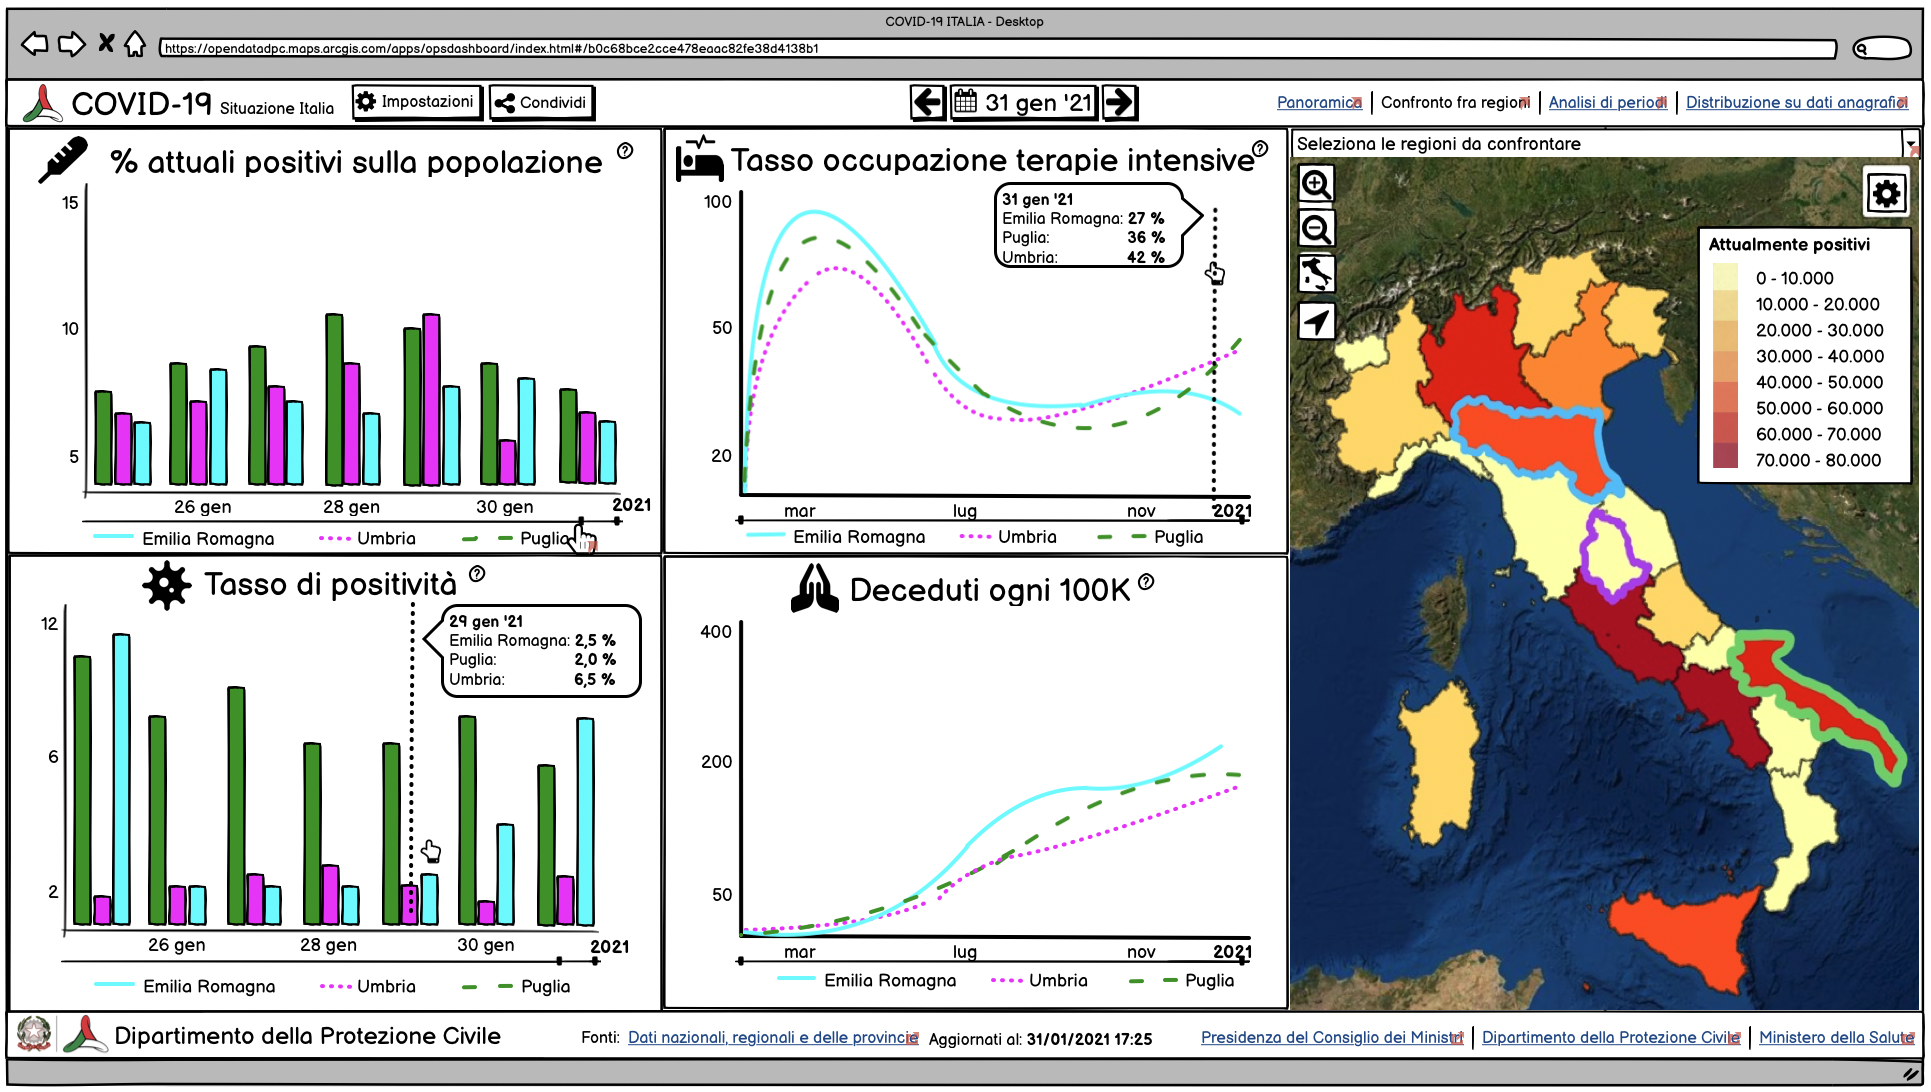
\includegraphics[width=1\columnwidth]{wireframes/confronto-regioni}
    \caption{Schermata ``Confronto fra regioni''.}\label{fig:confronto-regioni}
\end{figure}
La schermata ``Confronto fra regioni'' è raggiungibile cliccando sul link in alto a destra. In questa schermata è possibile selezionare una o più regioni per confrontare alcune metriche mediante dei grafici. La selezione avviene mediate una lista \textit{ComboBox} posizionata al di sopra dell mappa, come mostrato in~\ref{fig:seleziona-regione}, oppure cliccando direttamente sull'area della regione che si vuole aggiungere al confronto. Le regione selezionate sono indicate tramite una spunta (\checkmark) e i loro confini sono colorati con gli stessi colori assunti poi nei grafici.

\begin{figure}[H]
    \centering
    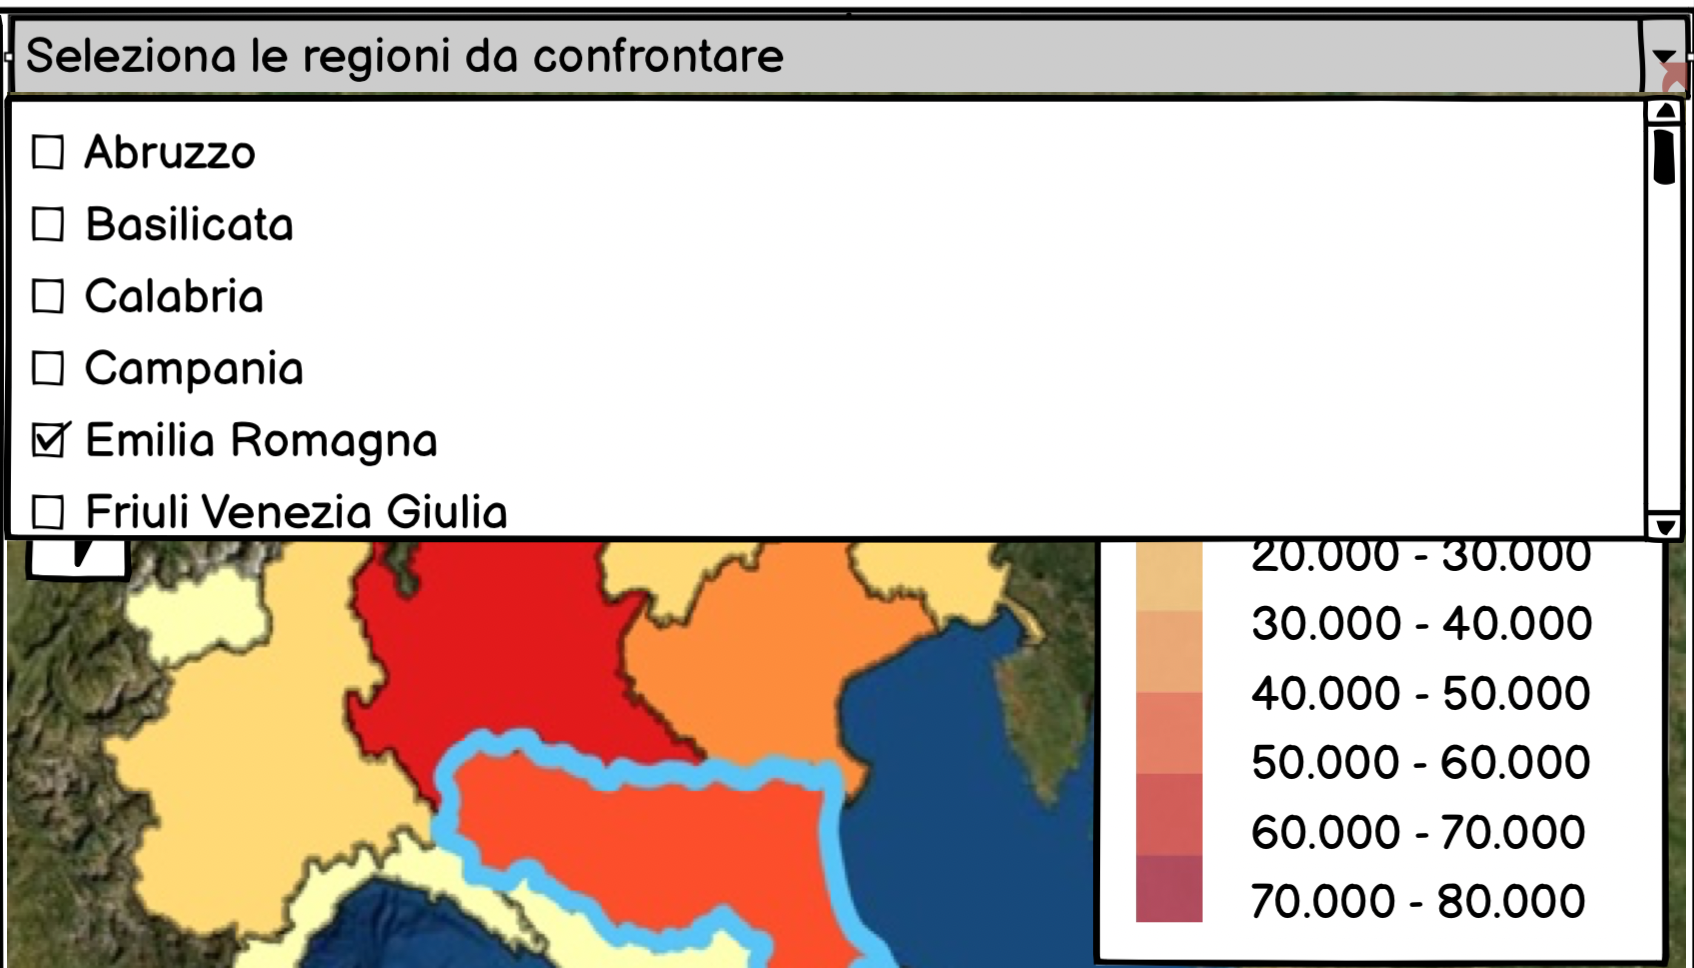
\includegraphics[width=0.5\columnwidth]{wireframes/seleziona-regione}
    \caption{ComboBox per la selezione delle regioni.}\label{fig:seleziona-regione}
\end{figure}

I grafici presenti sulla parte sinistra della schermata, di cui~\ref{fig:esempio-grafico-confronto-regioni} ne è un esempio, sono formati da diverse linee, una per regione selezionata; ogni regione è riconoscibile tramite colore e tramite tratteggio, queste due caratteristiche sono uniche per ogni regione in modo che anche chi ha difficoltà a riconoscere i colori possa comprendere il grafico.

\begin{figure}[H]
    \begin{subfigure}[b]{0.5\textwidth}
        \centering
        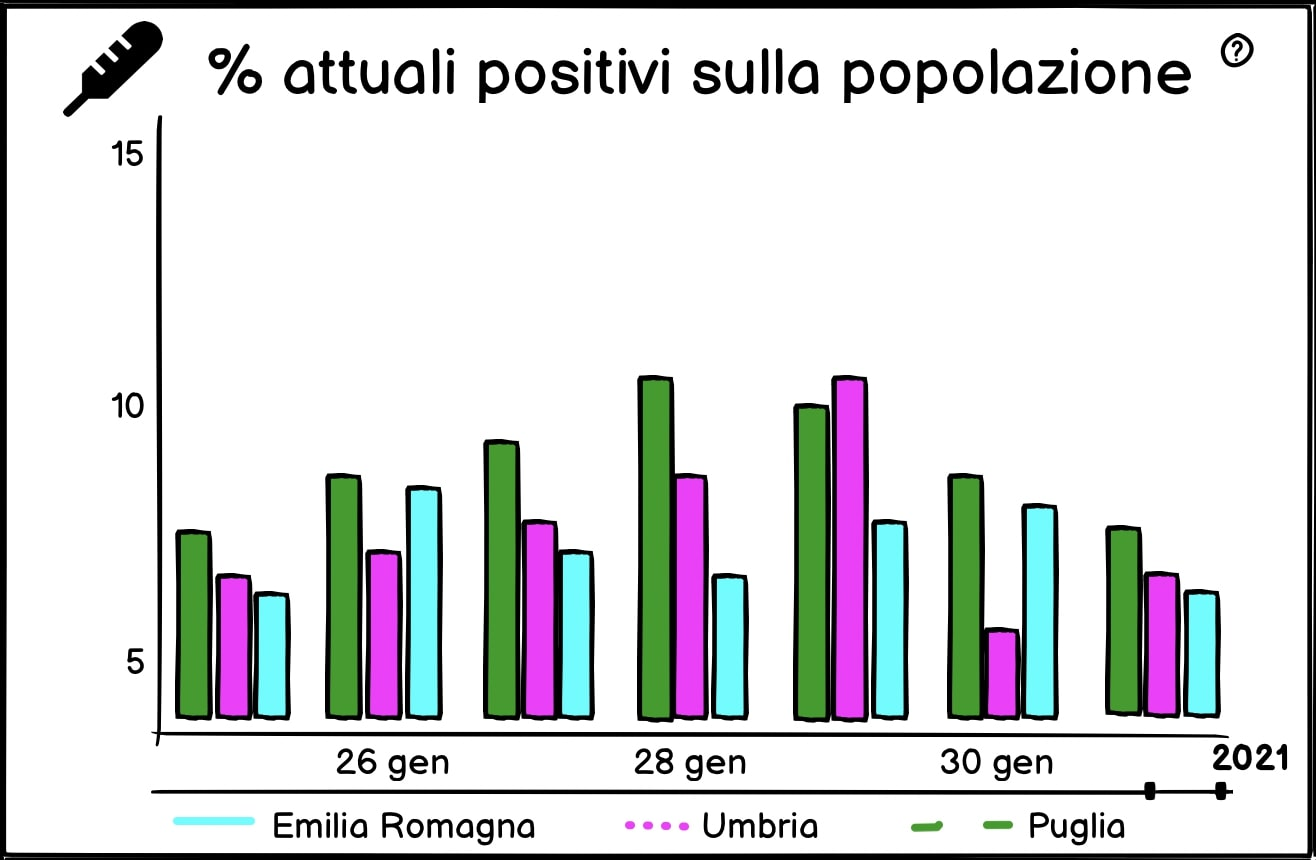
\includegraphics[width=1\textwidth]{wireframes/esempio-grafico-confronto-regioni-poco-tempo}
        \caption{Grafico per il quale è stato selezionato un range temporale di breve durata.}\label{fig:esempio-grafico-confronto-regioni-poco-tempo}
    \end{subfigure}
\hfill
    \begin{subfigure}[b]{0.5\textwidth}
        \centering
        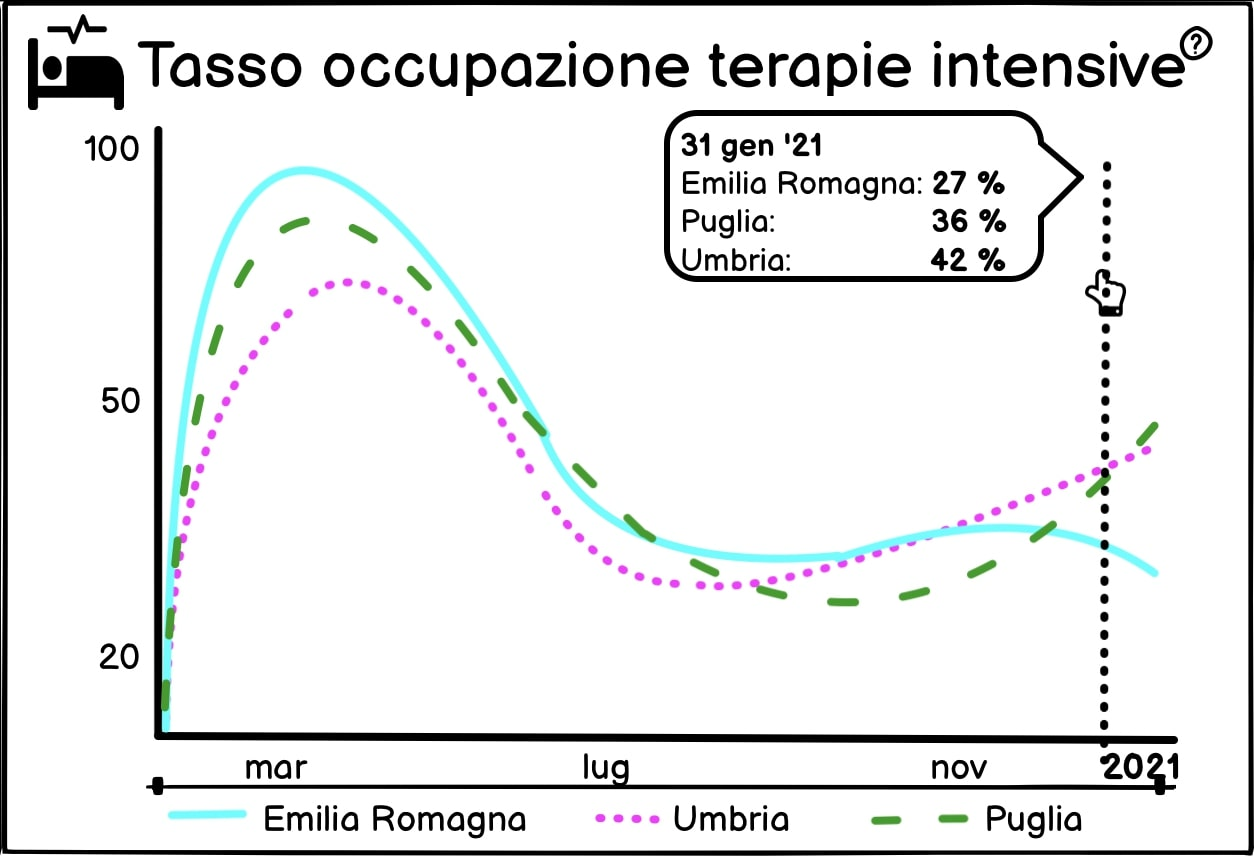
\includegraphics[width=1\textwidth]{wireframes/esempio-grafico-confronto-regioni-molto-tempo}
        \caption{Grafico per il quale è selezionato un range temporale di lunga durata.}\label{fig:esempio-grafico-confronto-regioni-molto-tempo}
    \end{subfigure}
    \caption{Differenze tra un grafico in cui è selezionato un range di tempo di breve durata e uno di lunga.}\label{fig:esempio-grafico-confronto-regioni}
\end{figure}

\subsubsection{Analisi di periodi}\label{ss:analisi-di-periodi}
\begin{figure}[H]
    \centering
    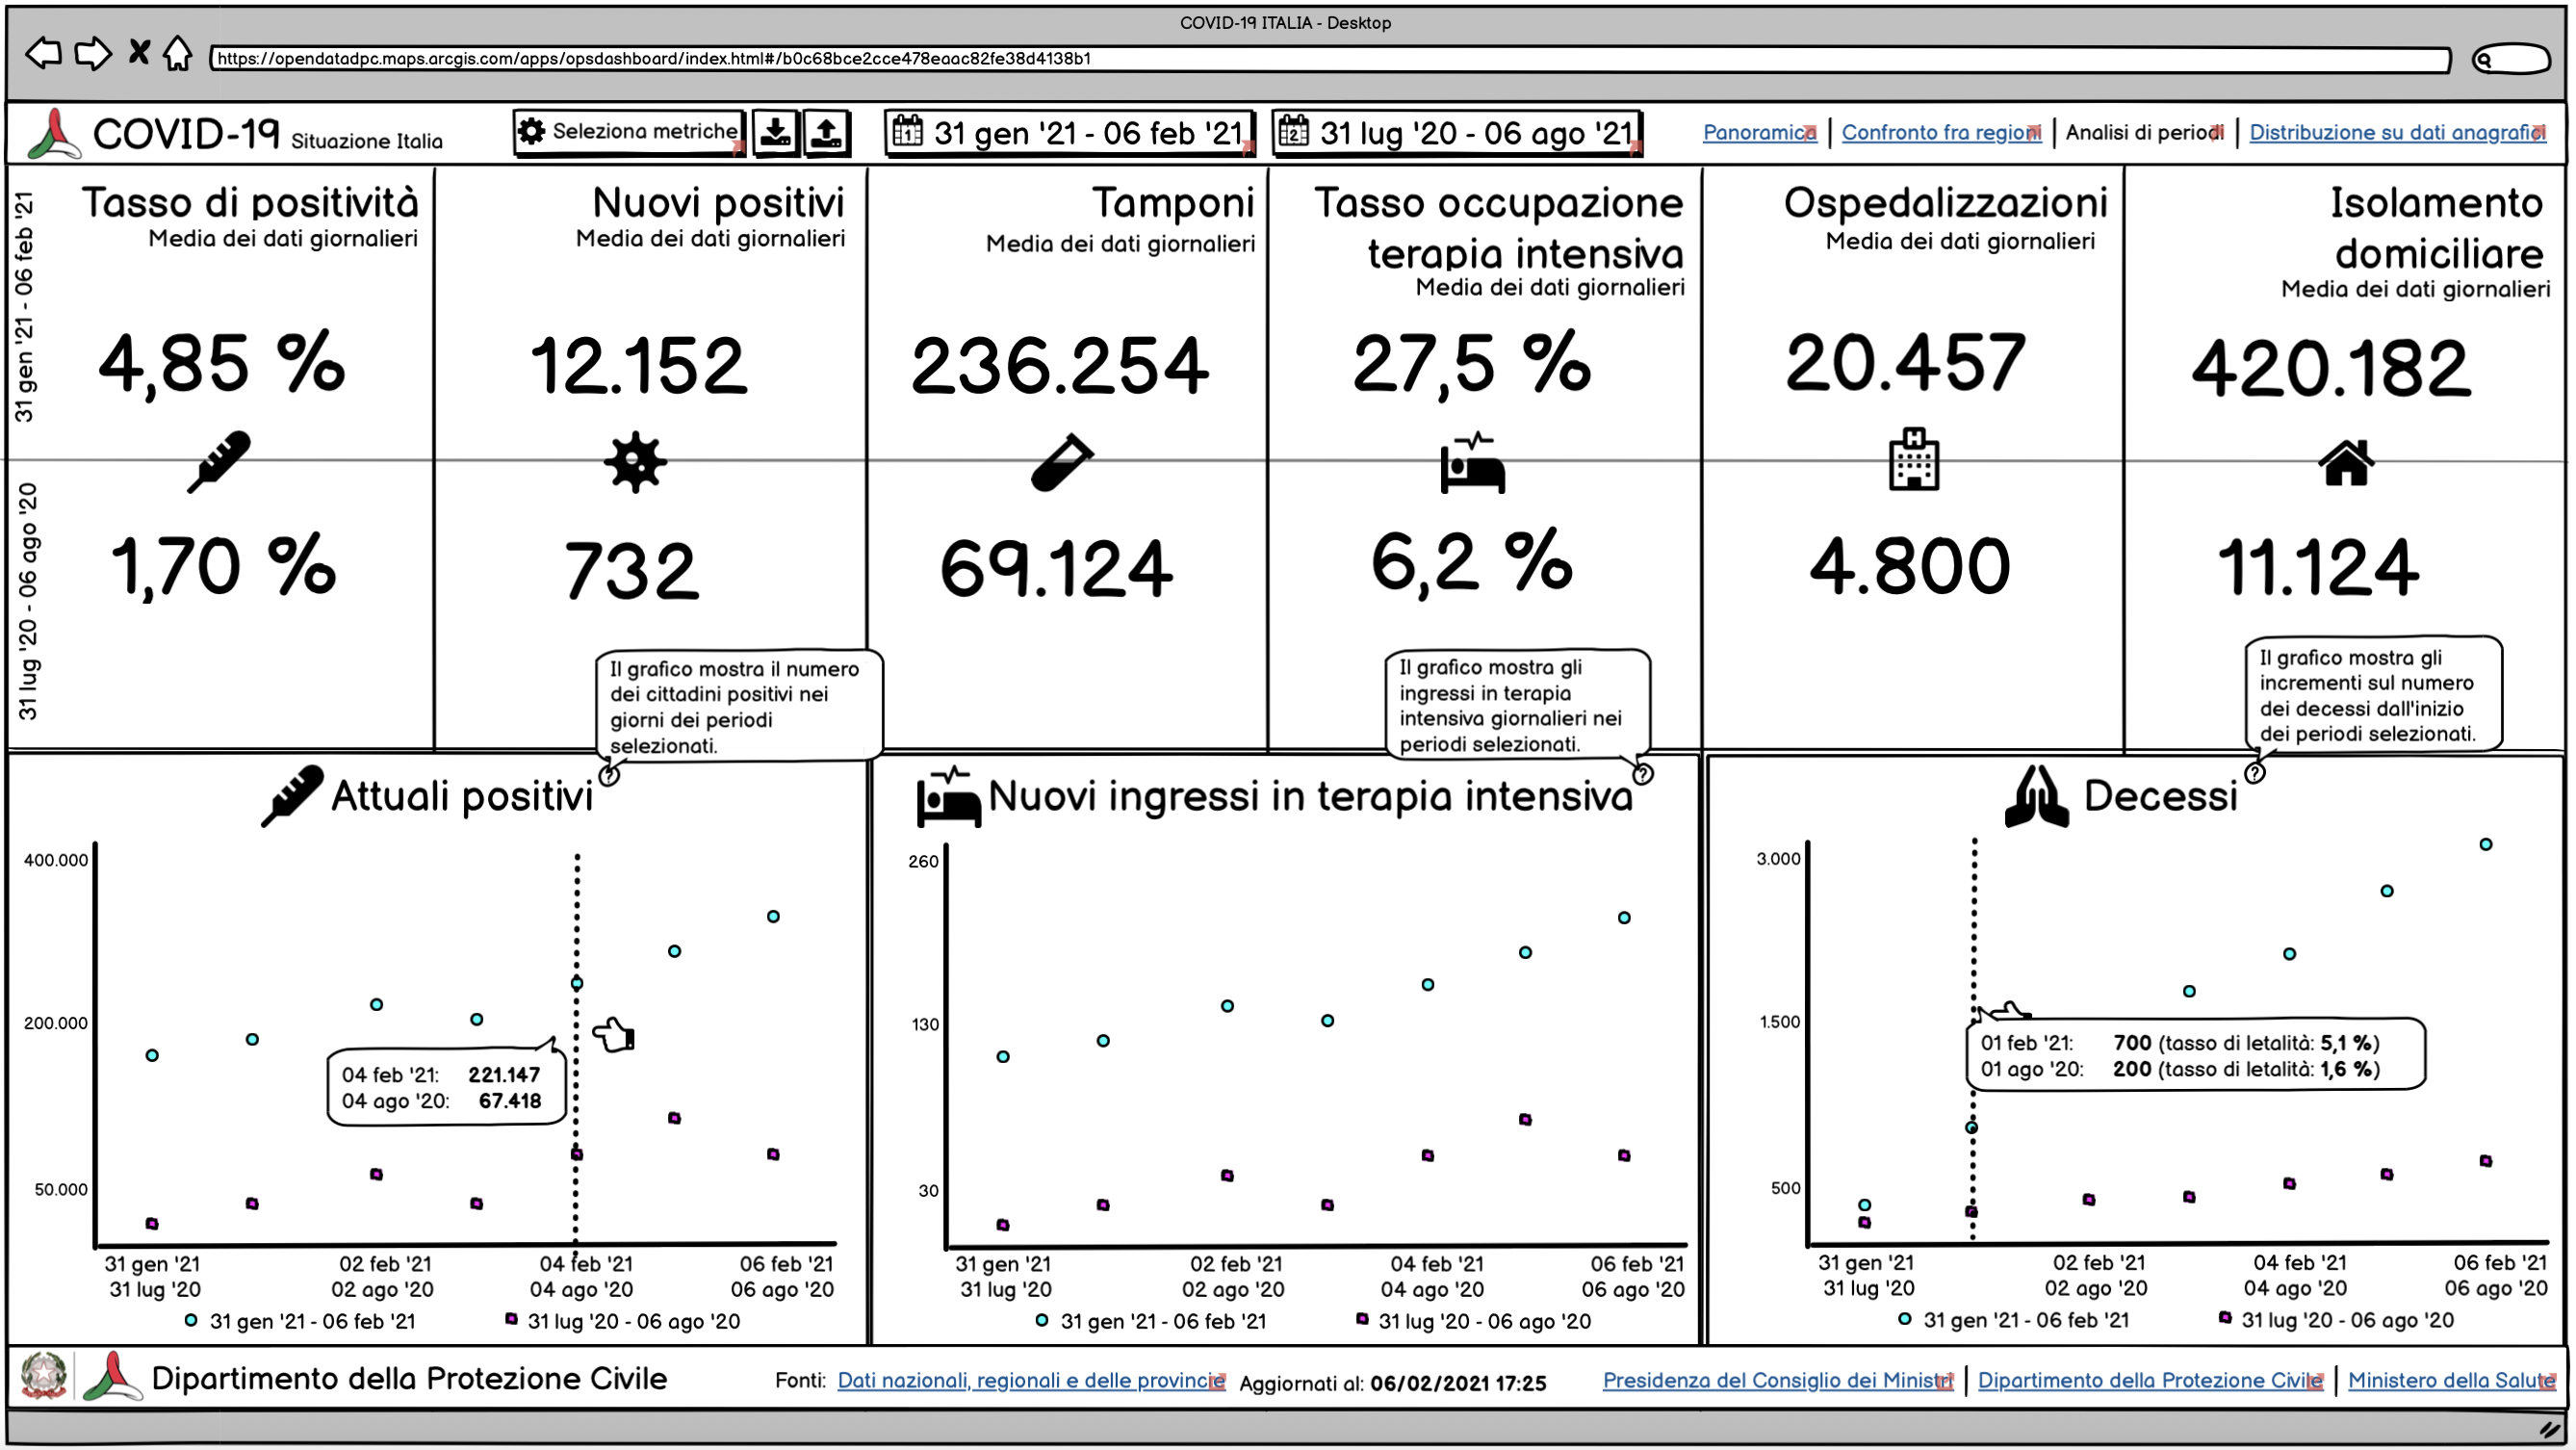
\includegraphics[width=1\columnwidth]{wireframes/analisi-periodi}
    \caption{Schermata ``Analisi di periodi''.}\label{fig:analisi-periodi}
\end{figure}
La schermata ``Analisi di periodi'' è raggiungibile dal link in alto a destra. In questa schermata è possibile analizzare l'andamento della pandemia per uno o due periodi, in quest'ultimo caso si possono anche confrontare le diverse metriche che la schermata mostra.\\
La schermata può, per semplicità essere divisa in due fasce: nella fascia superiore vi è una sottospecie di tabella in qui sulle righe ci sono i periodi temporali che si vogliono analizzare, mentre, sulle colonne ci sono le metriche. In questo modo è semplificato il confronto tra periodi. In questo caso i valori mostrati sono valori medi rispetto all'intero periodo indicato.\\
Nella parte inferiore della schermata trovano spazio tre grafici; questi grafici, sull'asse delle X riportano i giorni dei periodi temporali che si stanno analizzando così da permettere un più semplice confronto tra i periodi temporali.

\subsubsection{Distrubuzione su dati anagrafici}\label{ss:distribuzione-su-dati-anagrafici}
\begin{figure}[H]
    \centering
    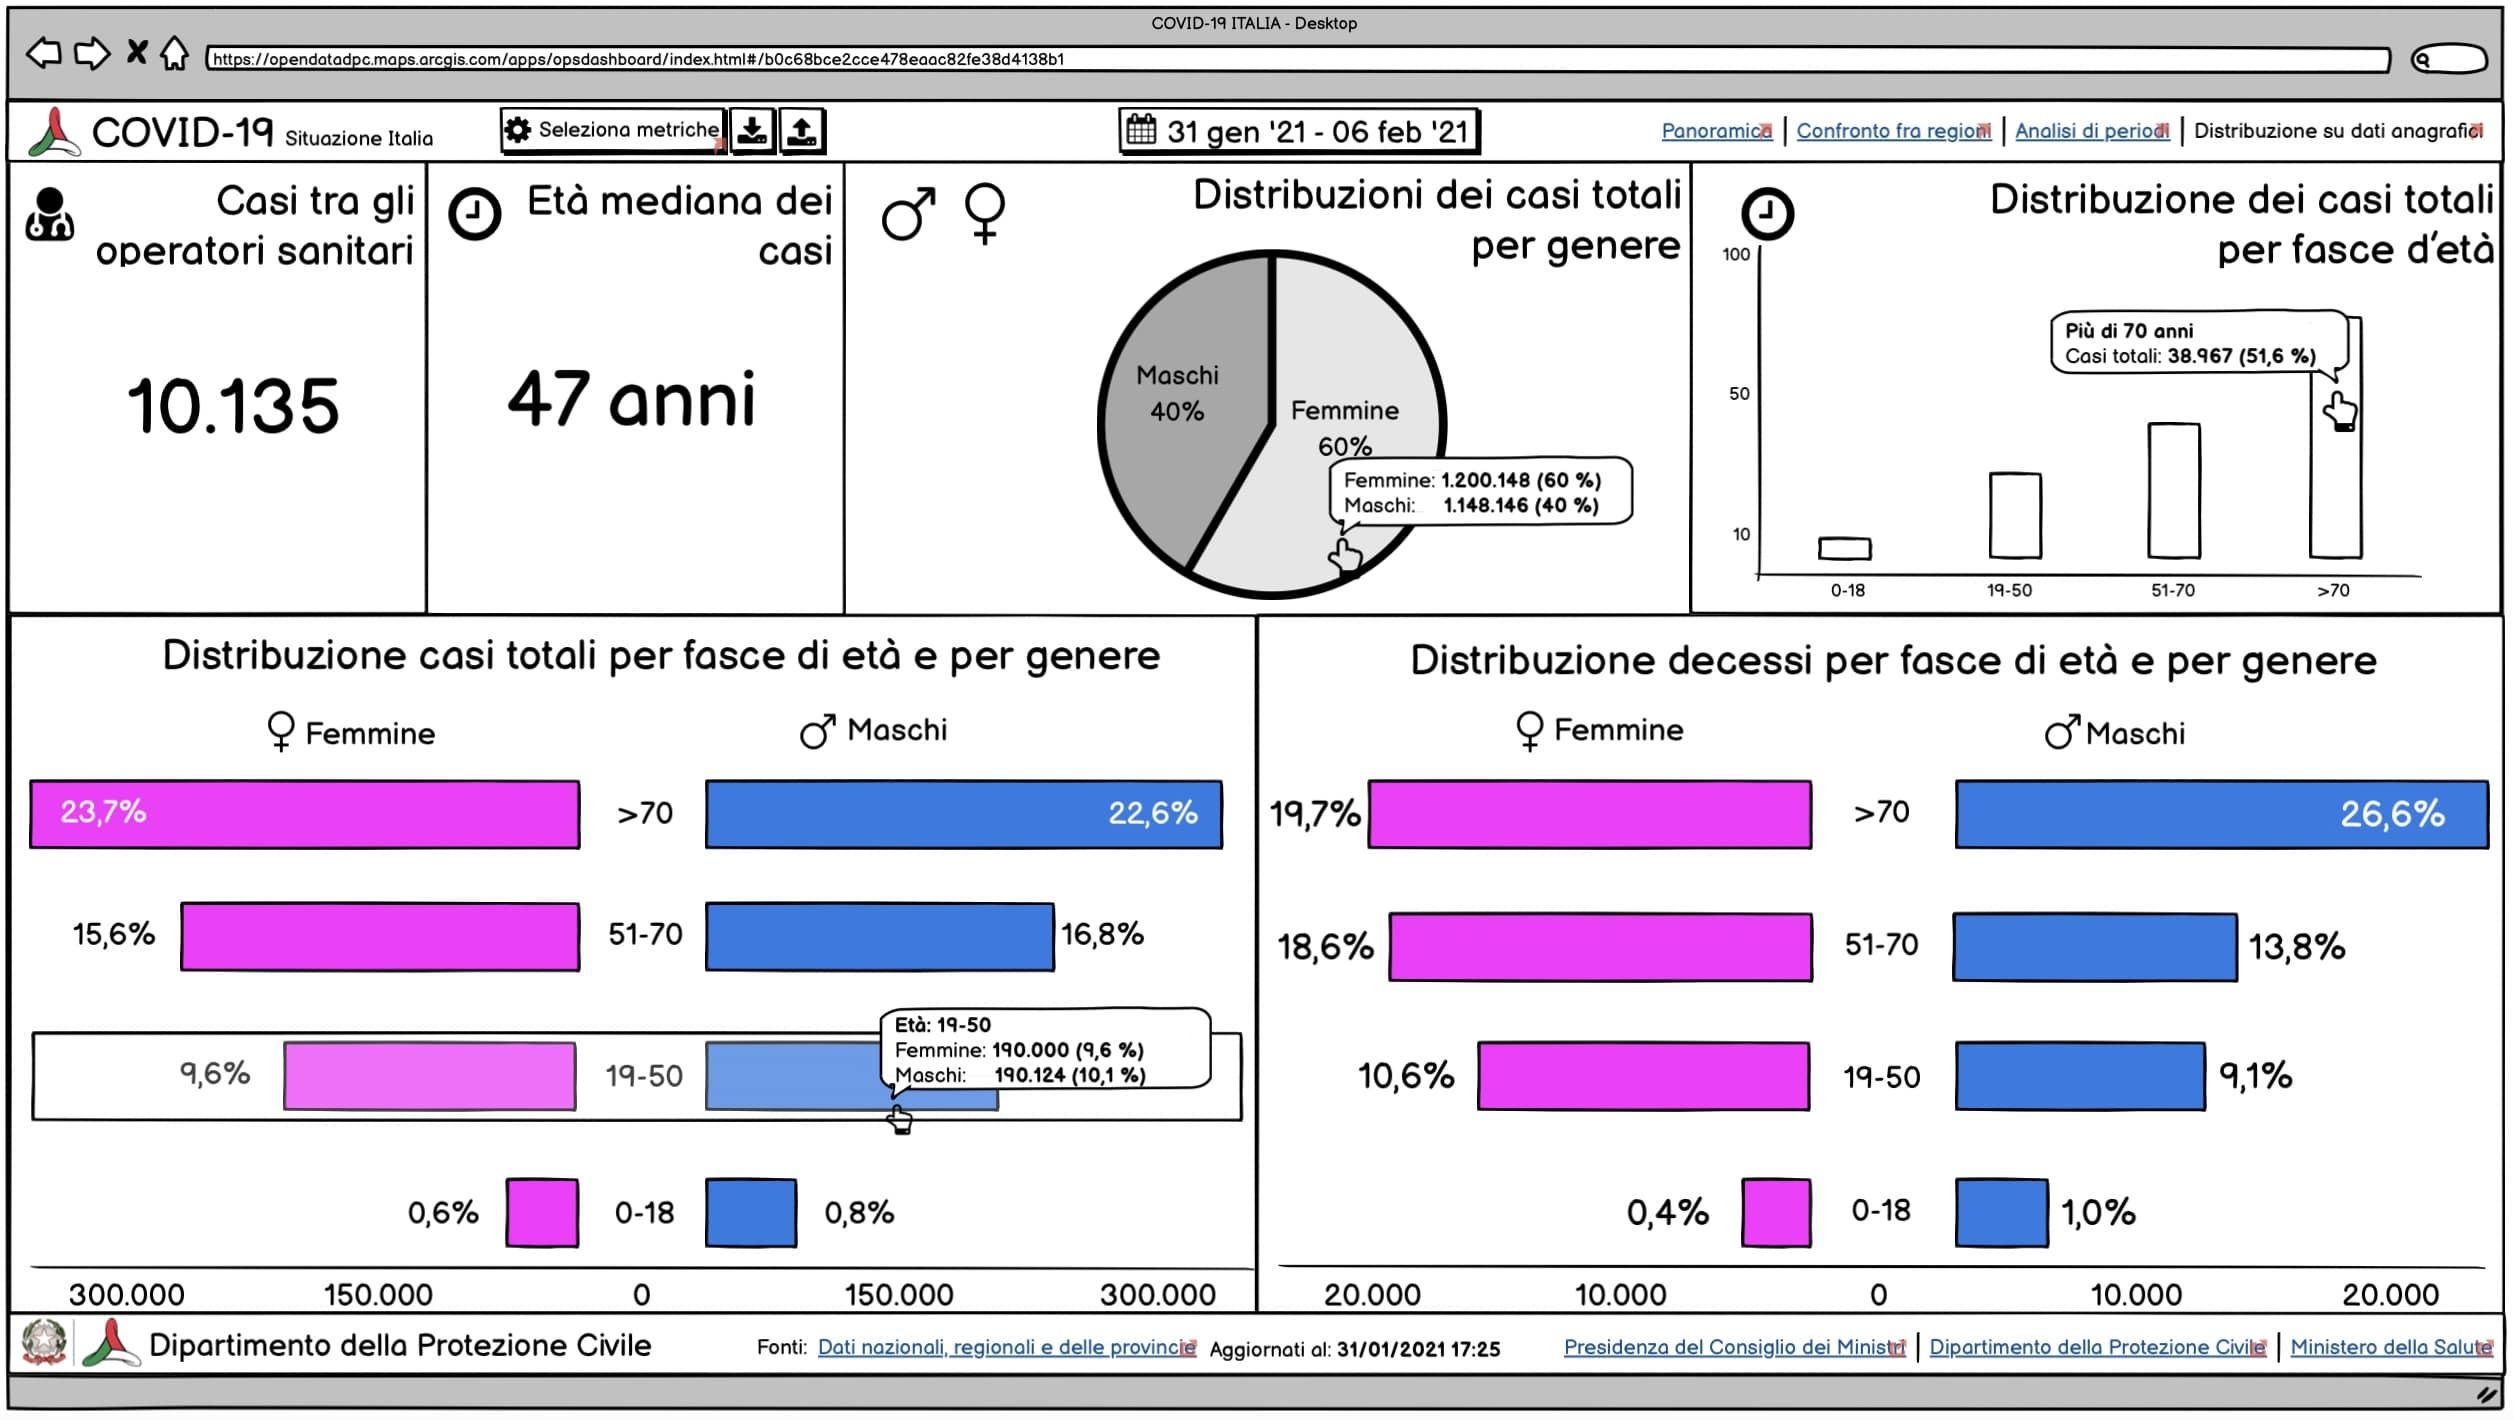
\includegraphics[width=1\columnwidth]{wireframes/distribuzione-dati-anagrafici}
    \caption{Schermata ``Distribuzione sui dati anagrafici''.}\label{fig:distribuzione-dati-anagrafici}
\end{figure}
La schermata ``Distribuzione sui dai anagrafici'' è raggiungibile dal link in alto a destra. In questa schermat è possibile analizzare come i numeri della pandemia si distribuiscano sulla popolazione in base all'età, al genere e al tipo di impiego. Questo viene fatto tramite box con numeri, areogrammi e istogrammi.

